% \documentclass[11pt,letterpaper]{article}
\documentclass[letterpaper,11.5pt]{scrartcl}
% \documentclass[11pt]{report}
% \documentclass{report}
% \documentclass{book}
\usepackage[bookmarks, hidelinks]{hyperref}
\usepackage[chatter]{rotating}
\usepackage{amssymb,amsmath}
\usepackage[title]{appendix}
% \usepackage{fullpage}
\usepackage{tabulary}
\usepackage{tabularx}
\usepackage{float}
% \usepackage[margin=0.50in]{geometry}
\usepackage[margin=1.00in]{geometry}

\usepackage{caption}
\usepackage{booktabs}
\usepackage{pslatex}
\usepackage{apacite}
\usepackage{subcaption}
\usepackage{pgfplots}
\usepackage{wrapfig}
\usepackage[english]{babel}
\usepackage{lmodern}
\usepackage{setspace}
\doublespace
% \usepackage{url}
\usepackage{bigfoot}
\usepackage[export]{adjustbox}
\setlength\intextsep{0pt}

% Colored comments 
\usepackage{color}
\definecolor{myorange}{RGB}{240, 96, 0}
\newcommand{\mt}[1]{{\textcolor{myorange} {({\tiny MT:} #1)}}}

\definecolor{myblue}{RGB}{30,144,255}
\newcommand{\jhj}[1]{{\textcolor{myblue} {({\tiny JHJ:} #1)}}}

\definecolor{mypurple}{RGB}{148,0,211}
\newcommand{\cm}[1]{{\textcolor{mypurple} {({\tiny CM:} #1)}}}

\definecolor{mygreen}{RGB}{26, 153, 51}
\newcommand{\ps}[1]{{\textcolor{mygreen} {({\tiny PS:} #1)}}}


\usepackage{graphicx}

\title{Uncertainty in the evolution of social learning}

\author{{}}

\begin{document}
\maketitle

\newcommand{\pisub}[1]{\pi_{\mathrm{#1}}}
\newcommand{\pilow}{\pisub{low}}
\newcommand{\pihigh}{\pisub{high}}
\newcommand{\piI}{\langle \pisub{I} \rangle}
\newcommand{\piS}{\langle \pisub{S} \rangle}

\newcommand{\meanvar}[1]{\langle #1 \rangle}
\newcommand{\meansl}{\meanvar{s}}
\newcommand{\meanpi}{\meanvar{\pi}}
\newcommand{\meansoc}{\meanvar{\pi_\mathrm{S}}}
\newcommand{\meanasoc}{\meanvar{\pi_\mathrm{A}}}
\newcommand{\meanT}{\meanvar{T}}

\begin{abstract}

Social learning is essential to survival. It is likely to evolve when it is more
efficient than asocial, trial-and-error learning. The consensus in cultural
evolutionary theory holds that some amount of environmental variability and
uncertainty about the best decisions are necessary for social learning to evolve.
However, current models for the evolution of social learning tend to conflate forms
of uncertainty, and rarely consider different ones in tandem. Moreover, many models
are limited by considering only two possible behaviors and environmental states.
Here we use evolutionary agent-based modeling to improve on these shortcomings. We
model a time-varying environment with dozens of possible behaviors performed by
agents engaging in individual and social learning. We show that ambiguous payoffs,
larger possible decision sets, and shorter agent lifespans sometimes increase social
learning prevalence, as expected. However, we also find that, under some conditions,
these forms of uncertainty can select against social learning.
\end{abstract}

\section{Introduction}

Social learning is essential to human and other species' everyday life and survival.
It allows individuals to solve problems when acquiring information from others is more efficient than learning
on one's own~\cite{Laland2004}. Theory predicts that social
learning should be favored in contexts with greater
uncertainty~\cite{BoydRicherson1985,Henrich1998}, and this prediction has received some empirical support~\cite{McElreath2005,Kendal2018}. 
However, the meaning of the term ``uncertainty'' is not always clear, and often conflates environmental variability, spatial heterogeneity, and ambiguity or uncertainty about payoff structure. 
Moreover, most models of the evolution of social learning ``blackbox'' key 
cognitive learning processes that underlie it~\cite{Heyes2016}. 

In this paper we use agent-based modeling to compare the effect of
different sources of uncertainty on social learning
by ``unblackboxing'' typically abstracted-out model components 
of environmental variability, payoff structures and
agent life histories, and  learning mechanisms. ``Uncertainty''  
means variability where the probabilistic structure is unknown. %cannot be learned.
Uncertainty increases when payoffs are more similar across behaviors, when
environmental variability increases, when the number of possible behaviors
increases, and when lifespan decreases.  In this paper we show that more ambiguous
payoff structures and shorter lifespans sometimes do lead to greater reliance on
social learning---however, we also identify and explain cases where greater
uncertainty leads to less social learning due to the possibility that social
information is misleading.  We thus conclude that many predictions made by previous
models of the evolution of social learning are likely overgeneralized.
%~\cite{Yarkoni2021}. 

\subsection{Social Learning}

Social learning, as we consider it here, occurs whenever an individual acquires a behavior by observing another individual. This need not require explicit instruction, and is, in fact, widespread across a broad range of nonhuman 
taxa~\cite{Kendal2018,Allen2019}. Importantly, social information can be inherited both
from parents --- i.e., via \emph{vertical transmission} like genetic information --- and
from others in the same generation --- i.e., via \emph{horizontal transmission}
\cite{CavalliFeldman1981}. The joint action of vertical and horizontal transmission
gives rise to qualitatively different evolutionary dynamics. For example,
inter-generational environmental change will affect the adaptive value of genetic
information and vertically-transmitted cultural information more than information
that is horizontally transmitted. We include both horizontal and vertical transmission pathways in our
model. For simplicity, we ignore oblique transmission in which non-parental members
of the previous generation are observed.

Environmental variability has been seen as a key selective force in shaping social learning starting with the first formal models of cultural evolution~\cite{CavalliFeldman1981,BoydRicherson1985}.
Totally stable environments will not favor learning mechanisms because information can become genetically hardwired, while  extreme environmental instability will degrade the value
of social learning as information becomes rapidly outdated~\cite{Feldman1996}. This suggests that an intermediate degree of environmental predictability will favor social learning. Strategies can also evolve to mitigate the risks of relying on outdated social information by weighing more heavily information from others who more recently acquired it~\cite{Rendell2010}.

Uncertainty has also been modelled as arising from other aspects of the environment. 
For example, \citeA{Perreault2012} vary the ambiguity of the environmental cue individuals get through individual learning about the state of the world. Perhaps not surprisingly, the more ambiguous the asocial information, the greater the selection for weighing social information heavily. Alternatively, uncertainty about the optimal behavior has been modelled by increasing the number of cultural traits to choose from. 

Empirical research supports some of these theoretical predictions. Organisms flexibly use social learning as a function of the ambiguity of the environmental cue and of other environmental features that are often subsumed under the rubric of ``uncertainty.''
While some studies explicitly impose a cost whenever participants use asocial
information \cite{Morgan2012,Atkisson2012}, 
others allow the costs of each strategy to emerge as a function of task structure and assess its consequences for learning strategies. 
For example, when participants received equivocal private information about the best investment to make in a lab game,
they were more likely to rely on social information to make their choice~\cite{Toelch2013}. 
\citeA{McElreath2005} developed a similar experiment where participants ``pulled'' virtual slot machine arms (often called ``bandits''), each yielding stochastic payoffs. Participants relied more on social learning when the bandits had higher-variance payoffs, and when the highest-paying bandit changed more frequently. 
The number of options to choose between can also increase uncertainty about the optimal choice, and has been shown to increase participants' reliance on social learning \cite{Muthukrishna2016a}. 

Thus existing theoretical work and the empirical evidence seem to support that various forms of uncertainty favor the evolution of social learning. However, uncertain outcomes are operationalized in different ways across models, and any given model tends to focus on only one or two forms of uncertainty at a time. Our agent-based modeling approach enables us to explicitly specify different forms of uncertainty independently in order to understand which of these environmental factors particularly favor the evolution of social learning. Simultaneous modelling also allows us to examine their interaction. We first attempt conceptual replications of previous models' findings, and then examine where they diverge.

\subsection{Research overview}

Computational agents in our model face a problem: every time step they perform
one of several behaviors, with each behavior represented by a ``bandit'' that
pays off 1 or 0 with some probability. One of these behaviors (the optimal
behavior) pays off with a higher probability than all the others.
Agents decide which behavior to 
perform based either on a success-biased observation 
of a peer's behavior (social learning) or based on their own observations (asocial learning).
Agents then update their memory of expected payoffs for each behavior 
when they receive a payoff from their chosen
action. Within this framework we have four mechanisms by which we operationalize 
and vary uncertainty:
(1) the expected payoffs of the optimal behavior and all the rest---when payoffs
are nearly identical, uncertainty in the form of ambiguity increases; (2) the
environmental variability, i.e., the probability that the optimal behavior 
changes between generations; (3) the number of possible behaviors the environment allows---which
behavior is optimal is more uncertain when there are more possibilities; and (4)
 agent lifespan---agents experience fewer learning opportunities and die more uncertain about which behavior
is optimal when their lifespan is shorter. 

The primary outcome measure of our
model is the average difference between the frequency of (horizontal) 
social learning and the frequency of asocial
learning across all agents. If social learning is more prevalent than asocial
learning this suggests that the optimal behavior is more likely found
by copying peers than by trial-and-error search.
Conversely, when asocial learning is more prevalent, this suggests social information
is likely to be misleading. 
When social and asocial learning are 
equally prevalent this means there is no discernible advantage to either, i.e.,
the agents have weak priors on which channel provides more reliable information. 
Each agent has its own social learning frequency that it inherits from its
parent (haploid reproduction) with mutation, so evolution selects for,
or computes~\cite{Smaldino2013}, the optimal
social learning frequency.

Using our model we found that increased uncertainty sometimes
led to increased reliance on social learning, as expected from prior literature. However, we also find cases where increased uncertainty decreased agents' reliance on social learning
due to increased uncertainty that made social information less reliable, thereby
increasing reliance on asocial learning.

\section{Model}

We developed an agent-based model of a society of $N$ individuals who each must decide
which of $B$ behaviors to perform at each time step. Each behavior is a ``bandit'',
a common modelling and experimental approach for representing behaviors with
probabilistic payoffs~\cite{SuttonBartoBook, McElreath2005,Rendell2010,Schulz2019}. %Bandits are like  slot machines in a casino~\ref{fig:behaviorSelection}.
Each behavior $b$ yields Bernoulli payoffs: payoff of 1 with probability $\pi_b$ and zero payoff
with probability $1 - \pi_b$; 
$\pi_b$ is therefore also the expected payoff of behavior $b$. Agents must
decide which behavior to perform at each time step. To do this, agents 
use an explore-exploit strategy to sometimes try the most profitable behavior
they know about, and other times try alternatives that may pay off more reliably. 

We operationalized uncertainty in four different ways: 
(1) payoff ambiguity, $A_\pi$, which measures the difference
between the optimal expected payoff behavior $\pisub{high}$ and the expected payoff
of the other behaviors, $\pisub{low}$; 
(2) environmental variability, $u$, the probability the optimal behavior changes from one generation to another; 
(3) the number of possible behaviors, $B$; and 
(4) the lifespan, or time steps per generation, $L$. 

We ran the simulation until agents evolved to be all social or all asocial 
learners, or until 20k time steps was reached. Only 44 out of 396k trials
did not reach fixation (all social or all asocial). At
the end of each generation agents reproduce and then die off. 
Those selected to reproduce
pass on their boolean social learning trait, $s$, without mutation,
which specifes whether agents learn socially. We developed a series of
computational analyses where we systematically vary the uncertainty
variables and observe the average prevalence of social learning trait $s$
across agents and trials, which is our primary outcome measure, 
denoted $\meansl$. 

\subsection{Agents and their attributes}

In each time step, $N$ agents---autonomous problem solvers---select 
which behavior to perform based on their running tally of mean payoffs for 
each available behavior. %information (Figure~\ref{fig:behaviorSelection}). 
Agent $i$ tracks the mean payoff of each behavior $b$, denoted $\bar\pi_{ib}$, and
a \emph{count} of how many times it has performed each behavior, denoted $c_{ib}$.
$\bar\pi_{ib}$
is initialized to 0 for all $b$ at model initialization for
all agents, and after each generation for individual learner agents. Social
learning agents' $\bar\pi_{ib}$ is initialized as that of its teacher selected
through performance-biased oblique learning. Agent $i$'s accumulated payoffs
from performing several behaviors over their lifetime of $L$ time steps is
denoted $\pi_{i}$.

\begin{table}[h]
    \caption{Dynamic agent-level variables. Each has an implicit time dependence.}
    \label{tab:modelParameters}
    \centering %\hspace{-3em}
    \begin{tabular}{cp{2.5in}p{1.0in}} \toprule

        Attribute & Description & Initial value \\ 

        \midrule  

        $s_i$  & Social learner trait: 1 if agent $i$ is social learner; 0 otherwise & 0
        or 1 w/ equal prob. \\

        $\bar\pi_{ib}$ & ``Ledger'': mean payoffs acquired via behavior $b$ by $i$ 
                       & $B$-vector of floating-point zeros \\

        $c_{ib}$ & Count of how many times agent $i$ performed $b$ 
              & $B$-vector of integer zeros \\

        $\pi_i$ & Net payoffs accumulated by $i$ within generation
                                & 0.0 \\
        \bottomrule
    \end{tabular}
\end{table}
\subsection{Modeling uncertainty}

In our model uncertainty is a tunable consequence of four environmental features:
\begin{enumerate}
    \item 
      We vary the frequency at which the optimal behavior changes, which we call
      \emph{environmental variability}, $u$. At the start of each generation, with
      probability $u$, a new behavior is assigned a payoff of $\pisub{high}$ while all
      other behaviors are assigned a payoff of $\pisub{low}$. Otherwise, the same
      behavior remains optimal across generations. 
    \item We vary the latent expected payoffs yielded by the bandits. For simplicity,
      we assume that in any given environmental state, there is one optimal behavior that
      yields an expected payoff of $\pisub{high}$, while all other behaviors yield a 
      payoff of $\pisub{low} < \pisub{high}$. As $\pilow$ increases towards 
      $\pihigh$, uncertainty in the form of \emph{payoff ambiguity} also increases,
      making it more difficult, and less rewarding, for agents to determine which
      behavior is the optimal one.
    \item We vary the total \emph{number of available behaviors}, $B$, which is a
      source of uncertainty since agents are less likely to know which behavior yields high payoffs.  
    \item Finally, we vary number of behavioral events per generation, $L$. This can be viewed as the \emph{effective lifespan} of an agent.  Decreasing this lifespan effectively increases the importance of each event for acquiring payoffs. When lifespans are short ($L$ is small), agents experience greater uncertainty about which behavior is optimal given the fewer learning opportunities.
\end{enumerate}

\subsection{Dynamics and evolution}

Model dynamics can be split into three parts: initialization,
\emph{intra}generational behavior and payoff accumulation, and
\emph{inter}generational transmission of the social learning trait and oblique
learning (Figure~\ref{fig:IntraInterGenerationalDynamics}). 
The model runs that we analyze here were initialized with $N=100$ agents
to randomly have the social learner trait or not, with no accumulated payoffs, and
blank ``ledgers''. At each time step, agents select one of $B$ possible behaviors
to perform, accumulating a payoff of 1 if the bandit pays off, and 0 if it does
not---a bandit pays off with probability $\pihigh$ if it is the unique optimal
behavior, or with probability $\pilow$ if it is one of $B-1$ non-optimal
behaviors. Agents accumulate payoffs in this way for $L$ time steps in each
generation. At the end of each generation, $N=100$ agents are randomly selected with
replacement to reproduce (asexual, haploid reproduction), 
weighted by their net payoffs over the generation,
i.e., \emph{performance-biased} reproduction. Child agents then learn from 
one teacher, selected again via a form of performance bias: a child agent chooses
its teacher by first selecting a fully random subset of agents from the 
parent generation as potential teachers, then selecting the one with the 
greatest net payoffs among the subset. This process continues until agents
have become all social or all asocial learners, or when $20k$ time steps have
elapsed. 

\begin{figure}
  \caption{Model dynamics are composed of two major parts: first, agents perform
  behaviors for $L$ time steps in a single generation. Then agents reproduce
  randomly, with more successful agents being more likely to reproduce. Newly
  ``born'' social learner agents use success bias to select and learn from a chosen
  teacher. Then, all agents from the previous generation die off, all new agents
  begin a new generation, and the process continues until 1000 total time steps
  have elapsed. Agents are initialized as ``blank slates''. \mt{Can compress this
  into triptych. $M \rightarrow L$. Lighten grey background, remove outlines
around most or all components. Replace text in picture with A, B, C, and 
explain in caption.}}
  \label{fig:IntraInterGenerationalDynamics}
  \centering
    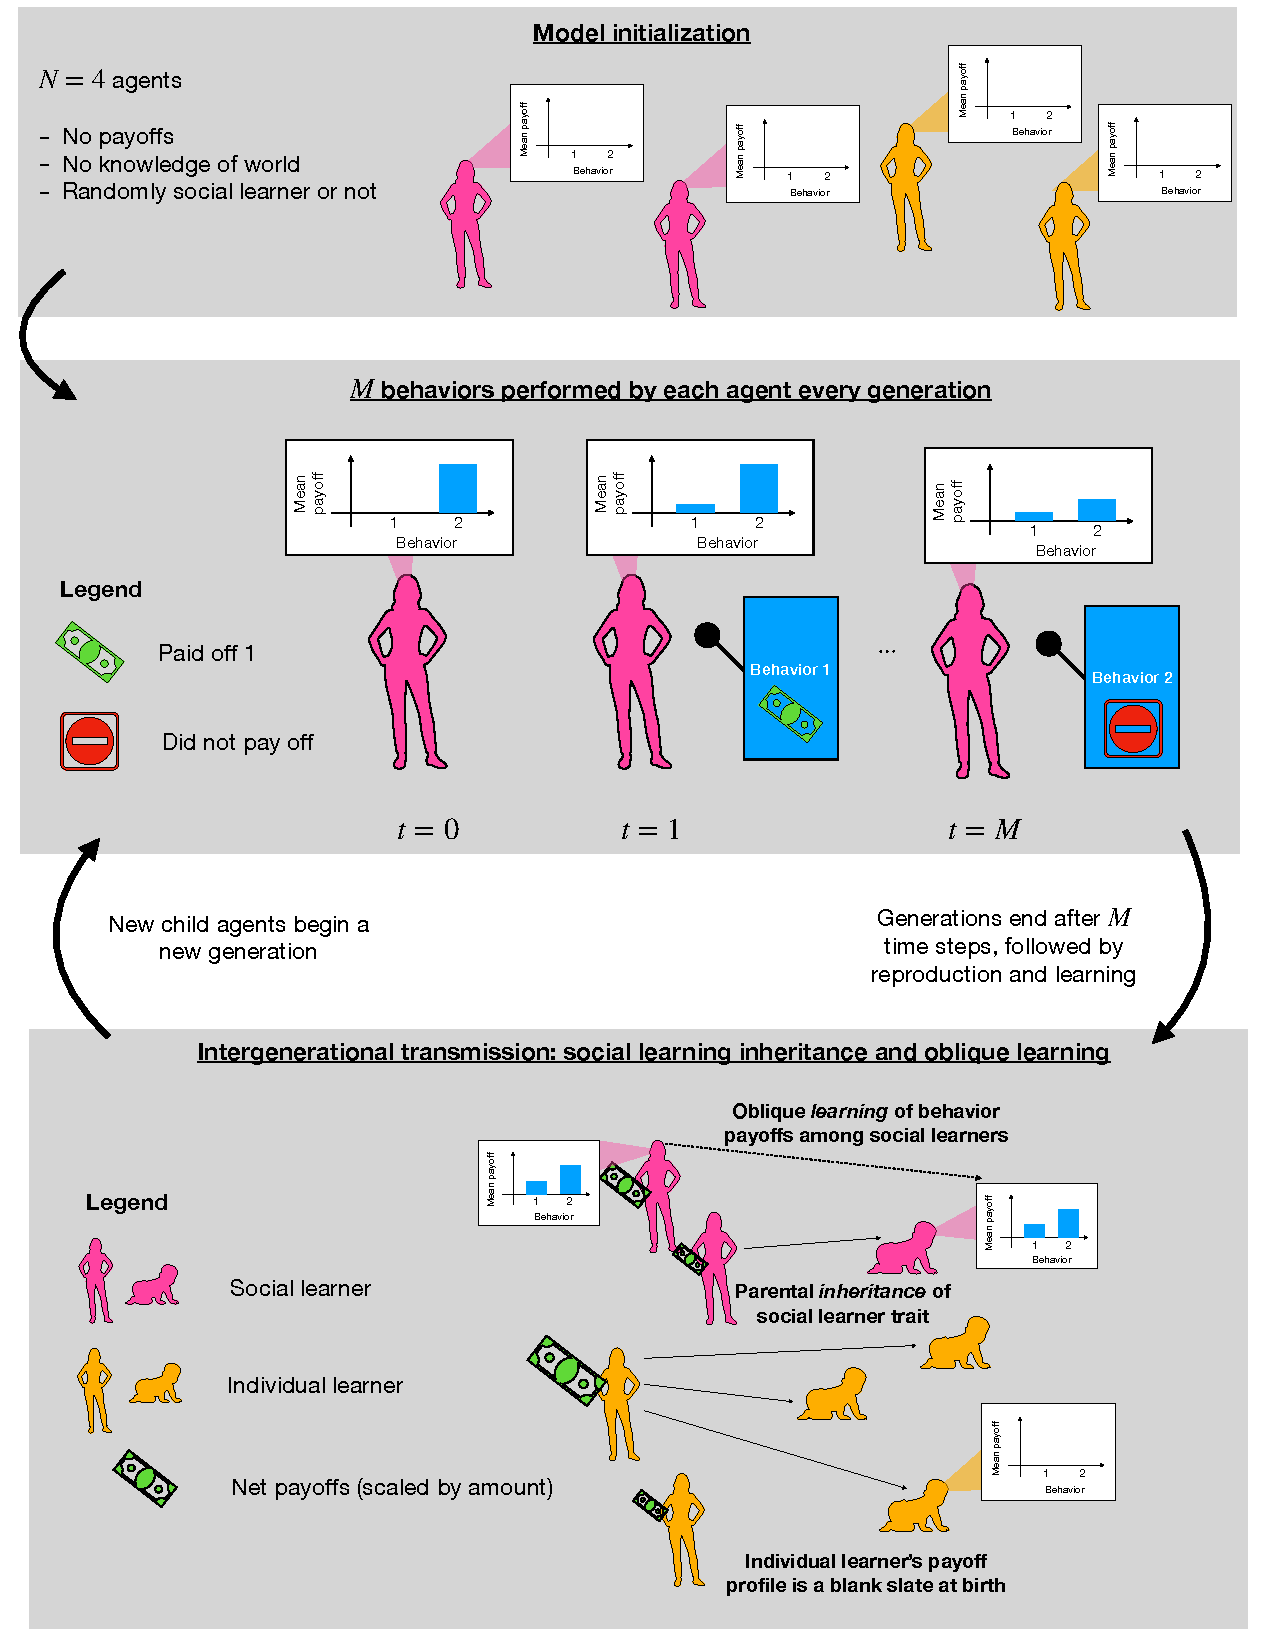
\includegraphics[width=0.9\textwidth]{Figures/IntraInterGenerationalDynamics.pdf}
\end{figure}


\subsubsection{Initialization}

Model initialization includes agent and environment initializations. Agents are
randomly initialized to have the social learning trait or not, with equal 
probability. Agent ``ledgers'' and behavior counts 
are uniformly initialized to the no-knowledge,
blank-slate case where all $\pi_{ib} = 0$ and $c_{ib} = 0$. Both the 
ledger and behavior count vectors have $B$ entries, one for each
behavior the environment affords. Net payoffs for
the generation are also initialized to zero. All agents are initialized with
the same softmax temperature, $\tau$, that guides their behavior selection 
to be either more exploratory (greater $\tau$) or more exploitative of
what agents believe to be the optimal behavior(s) (lesser $\tau$).

The environment is initialized to have $B$ behaviors with one of them selected
at random to be the optimal behavior, denoted $b^*$. Behavior $b^*$ is 
initialized to have a probability $\pihigh$ of paying off 1. All other behaviors
are initialized to have probability $\pilow$ of paying off 1. The modeler must
specify the environmental variability, $u$, and the number of time steps per 
generation, $L$. 

\vspace{2em}
\begin{table}[h]
    \caption{Global environmental and cognitive initialization parameters.
    \mt{TODO: Test more $N_\text{T}$ for sensitivity analysis}}
    \label{tab:modelParameters}
    \centering %\hspace{-3em}
    \begin{tabular}{cp{2.5in}p{1in}} \toprule

        Symbol & Description & Values tested (bold$=$default) \\ 

        \midrule  

        $B$       & Number of possible behaviors (represented by ``bandits'') 
                  & 2, 4, 10 \\

        $\pihigh$ & Probability that the unique optimal behavior pays off 1 
                & \textbf{0.9} \\

        $\pilow$ & Probability one of $B - 1$ non-optimal behaviors pays off 1 
                 & 0.1, 0.45, 0.8 \\ 

        $\tau$ & Softmax temp.; $\uparrow=$more exploration, $\downarrow=$more
                    exploitation 
               & 0.01, \textbf{0.1}, 1.0 \\
        
        $u$    & Probability optimal behavior changes between generations 
               & 0.0, 0.1, \ldots, 1.0 \\

        $L$    & Number of time steps per generation & 1, $B/2$, $B$, $2B$, $4B$ \\

        $N_T$    & Number of teachers to pool, from which best selected 
                 & \textbf{5}  \\

            
               
        \bottomrule
        \end{tabular} 
\end{table}


\subsubsection{Intra-generational behaviors and payoffs}

Each generation begins with agents initialized either by the $t=0$ initialization
outlined above, or initialized via inter-generational reproduction and learning,
described in detail below. Within generations, there is no social learning.
At each time step within a generation, agents select a behavior to perform
using the softmax algorithm, then update their ledgers $\bar\pi_{ib}$ and behavior
counts $c_{ib}$. If 
the chosen bandit pays off for an agent, its net payoff is incremented by one,
$\pi'_i \leftarrow \pi_i + 1$. This process continues for $L$ time steps, 
at which point reproduction, learning, and die-off occur, which re-initializes 
the next generation for performing $L$ behaviors selected via this same process.

At each time step, 
agent $i$ chooses behavior $b$ at random, with each behavior
weighted by the softmax function applied to that behavior's observed mean payoff
relative to all mean payoffs in the ledger,
\begin{equation}
  \Pr(i \text{ chooses behavior } b) = \frac{\exp(\bar\pi_{ib}
  / \tau) }{ \sum_{b=1}^B \exp(\bar\pi_{ib} / \tau)}.
\end{equation}  
Softmax behavior selection is a
biologically plausible model of behavior~\cite{Schulz2019} 
that enables agents to explore
alternative behaviors sometimes and exploit the best observed behavior other times,
in accordance with Luce's choice axiom~\cite{Luce1959},.
The parameter $\tau$ specifies how frequently alternative behaviors are
explored versus how frequently the best observed behaviors are 
exploited. Greater $\tau$ means more frequent exploration, lesser $\tau$ means
more frequent exploitation. We set $\tau = 0.1$ for
all computational analyses presented in the main paper. We 
 performed
sensitivity analyses and found a weak dependence on $\tau$ that does not affect our
main conclusions \mt{have run $\tau$ sensitivity checks, need to analyze them}.

When agent $i$ performs behavior $b$, $i$'s behavior count 
is incremented by 1, $c'_{ib} \leftarrow c_{ib} + 1$. Agent $i$'s ledger of mean 
payoffs are updated % from $\bar\pi_{ib}$ to $\bar\pi_{ib}'$
using exponential weighted averaging, 

\begin{equation}
  \bar\pi_{ib}' = \bar\pi_{ib} +
    \frac{\mathrm{Bandit_{b}(0, 1)} - \bar\pi_{ib}}{c_{ib}'},
\end{equation}
where 
$\mathrm{Bandit}_{b}(0, 1)$
is 0 or 1 depending on the result of the bandit draw for behavior $b$. 


\subsubsection{Inter-generational inheritance and social learning}

Every $L$ time steps, agents from the current generation reproduce, teach,
and die, while the next generation to perform the next $L$ time steps learns
from one teacher from the previous generation if they inherited the social 
learner trait. Inter-generational dynamics thus depend on 
two payoff-biased selection mechanisms: reproducer selection
and teacher selection. 

$N$ reproducers are sampled from the population with
replacement weighted by net payoffs, i.e., at each of $N$ draws for a parent,
\begin{equation}
  \Pr(\text{Agent $i$ chosen for reproduction}) = \frac{\pi_i}{\sum_{i=1}^N \pi_i}.
\end{equation}
\noindent
We sample with replacement to allow for more successful agents to have multiple
offspring. Child agents inherit their parents' social learning trait, so 
all social learner parents spawn social learner offspring, and parents lacking
the trait spawn offspring lacking the trait. 

Child agents with the social learning trait then must select and learn from a
teacher from their parent's generation, including possibly their parent.
Child agents give no preference to whether potential teachers are social 
learners. A child selects a teacher by first selecting a pool of $N_T = 5$ potential
teachers. Among this pool, each child selects the teacher with the greatest
net payoffs. In case of a tie the teacher is chosen at random from those with
the shared maximum net payoff. 

Social learner child agents each acquire their teacher's ledger, and all social
learner children behavior counts are reset to 1 to limit ledger values to be between
0 and 1. Child agents without the social learner trait have all ledger and behavior
count values re-initialized to 0. At this point the re-initialized child agents
engage in behavior selection and payoff accumulation described above. 


\subsection{Computational analyses and outcome measures}

We manipulated environmental uncertainty parameters described above, $u$,
<<<<<<< HEAD
$\pisub{low}$, $B$, and $L$, to examine their effects on our
main outcome measure, the mean prevalence of social learning $\meansl$, 
and supplemental outcome measures $\meanpi / L$ and $\meanT / L$. $\meanpi / L$ is the
mean net payoffs accumulated by agents at the end of each generation for the
final generation of agents, normalized by lifespan $L$. $\meanT / L$ is the 
mean time steps to convergence normalized by the lifespan of agents, i.e., the
mean number of generations until convergence was reached. Mean values were
caluculated across 100 model runs for each combination of uncertainty parameter values.
To test the effect of the uncertainty parameters, 
we initialized several model runs with
systematically varied uncertainty parameters, $u$, $\pisub{\mathrm{low}}$, $B$,
and $L$. We varied $u \in \{0.0, 0.1, \ldots, 1.0\}$ for each combination of
the following parameters:
$\pisub{low} \in \{0.1, 0.5, 0.8\}$, $B \in \{2, 4, 10\}$, and
$L \in \{1, B, 2B, 4B\}$ for $B=2$ and $L \in \{1, B/2, B, 2B\}$ for $B=4,10$.
=======
$\pisub{low}$, $B$, and $M$, to examine their effects on our
main outcome measure, the prevalence of social learning $s$. For each parameter setting
in our analysis we calculated the average value of $s$ at the final time step,
either at the maximum $T_{\text{max}}=20000$ across 1000 trials 
for each combination of uncertainty parameter values.

To analyze the effect of various forms of uncertainty on social learning 
prevalence in our Analysis, we initialized several model runs with
different uncertainty parameters $u$, $\pisub{\mathrm{low}}$, $B$,
and $M$. We varied $u \in \{0.0, 0.1, \ldots, 1.0\}$ for each combination of
the following parameters:
$\pisub{low} \in \{0.1, 0.45, 0.8\}$, $B \in \{2, 4, 10\}$, $L \in \{1, B/2, B, 2B\}$.

\subsubsection{Outcome variables}

Our primary outcome variable is the mean prevalence of the social learning
trait over $N=100$ agents over 1000 trials at the final time step of each trial,
denoted $\meansl$.
Typically at the final time step all agents either have the social learning
trait or do not (see Supplement for a presentation of time series collections
and histograms of outcomes for
a representative sampling of variables \mt{TODO}).
>>>>>>> 642146dabe76f30add3b2bafcd00edb4ef355867

\begin{table}[h]
    \caption{Outcome variables}
    \label{tab:outcomeVariables}
    \centering %\hspace{-3em}
    \begin{tabular}{cp{2.5in}p{1in}} \toprule

        Symbol & Description & Values \\ 

        \midrule  

        $\meansl$ & Mean social learning prevalence over agents and trials
                  & $\in [0.0, 1.0]$ \\

        $\meanpi / L$ & Mean payoffs accumulated in a generation normalized by
        lifespan & $\in [0.0, 1.0]$ \\

        $\meanT / L$ & Mean number of generations to convergence & Bounded above by 20k / 8\\
        \bottomrule
    \end{tabular}
\end{table}


\subsection{A note on relationship with standard RL formalism and models}

We presented our model as an agent-based model because that is
how we originally developed it. Howevever, we believe the model could be 
translated in a straightforward way where each action at time $t$, typically denoted
$a_t$, is to ``pull'' one of the $B$ bandits, and the policy $\pi$ would 
involve using the softmax function to weight random behavior
selection~\cite{SuttonBartoBook}. Because of the complication of two
relevant time intervals, intervals between actions and generational intervals, and
space limitations we do not try to put the entire model in standard RL terms.
\mt{Expand/improve.}

\section{Analysis}

To understand the effect of uncertainty parameters (1) environmental variability, $u$; (2) payoff
ambiguity that increases with $\pilow$; (3) number of behavioral options, $B$; and 
(4) generation length/agent lifespan, $L$, on the evolution of social learning, we analyze the results of
model runs across systematically varied parameter combinations.  We observed complex
outcomes where the effects of uncertainty parameters were highly dependent on one
another as measured by the mean prevalence of social learning, $\meansl$, across
trials for each parameter setting.  Increased environmental variability, $u$, 
tended to suppress social learning as expected from standard models of
social learning evolution. However, the shape of the decrease in $\meansl$ 
was not uniform (Figure~\ref{fig:evolutionOfSL}). 
Depending on the parameter settings, the critical value of $u$ at which social 
learning suppression began varied, as did the steepness of the decrease. 
We found that the location and width of the decrease in $\meansl$ is correlated
with the difference between the expected net payoffs of a population of all
social learners, $\meansoc$, and the expected net payoffs
of an all-asocial learner population, $\meanasoc$ (Figure~\ref{fig:meanNetPayoffs}). 
evolution does not always choose the theoretically highest payoff strategy,
and confirmed that evolution is more uncertain (i.e.\ selection is
weaker~\cite[p. 103]{BoydRicherson1985}) when $\meansoc - \meanasoc$ is small, 
where evolutionary uncertainty is measured by the 
average steps to model convergence, $\meanvar{T}$ (Figure~\ref{fig:steps}).

\subsection{Evolution of social learning under uncertainty}
<<<<<<< HEAD

We observed that different uncertainty contexts lead to different patterns in
the evolution and suppression of social learning. To understand the evolution
and suppression of social learning we inspected the social learning prevalence,
$\meansl$, which is the average of the frequency of social learning across
a model population over all trial model runs for a 4-tuple of uncertainty
values, $(u, \pilow, B, L)$.  We plot $\meansl$ on the y-axis 
over $u=0.0,0.1,\ldots,1.0$ on the x-axis in each plot, with nine plots total over
$\pilow=0.1,0.45,0.8$ and $B=2,4,10$, broken out by $L=1,B/2,B,2B$ within each plot
(Figure~\ref{fig:evolutionOfSL}). Across uncertainty scenarios, $\meansl$ monotonically
decreases $u$ increases, in accordance with classic cultural evolutionary
predictions~\cite{CavalliFeldman1981,BoydRicherson1985,Feldman1996}.  Therefore we compare
differences between uncertainty contexts in terms of the \emph{suppression of social learning}
over (increasing) $u$. 

Differences emerged in the suppression of social learning on two dimensions.
First there were systematic differences in the value of $u$ when social
learning first begins to be suppressed, i.e., where $\meansl$ first decreases. We show
in the following subsection that this occurs when $\meansoc$ approaches $\meanasoc$.
The second dimension of analysis is the width of the transition from 
maximal to minimal $\meansl$. In some cases, this width was less than 1, but
in many other cases the width was equal to 1, meaning that $\meansl$ 
decreased over all $u$. This indicated weak selection pressure since 
less than 0.001\% of all trials ended with all agents either social or asocial
learners. This is confirmed below by examining the average number of time steps
it took to reach fixation (agents all social or all asocial).

For now we will examine differences in the location and width of social 
learning suppression. \mt{In outline form while I work out each point}
\begin{itemize}
  \item 
    First, note that as $\pilow$ increases towards $\pihigh = 0.9$, social learning
    suppression widens, becoming linearly decreasing over $u$ with no $\meansl$
    reaching 1 or 0. This is due to weakened selection as the difference between
    social and asocial learning payoffs goes to zero.
  \item
    Second, as $B$ increases, note that social learning suppression 
    begins at increasingly high $u$. This is because it is increasingly worth
    the risk that a socially-learned ledger biases agents towards non-optimal
    behaviors when the number of choices increases. Furthermore, when $B$ is
    larger, one large ledger entry is not as misleading as when $B$ is smaller
    since there is more probability mass in the softmax vector's non-maximal
    behavior entries when $B$ is larger, and so alternatives to the socially
    learned ``best'' behavior will be explored more frequently.
  \item
    Finally, note that decreased lifespan both increases the location of 
    social learning suppression and the width of social learning suppression,
    with the extreme case of $L=1$ becoming linear and eventually flat compared
    to other values of $L$ as $\pilow$ and $B$ increase.
\end{itemize}
To support these explanations we need to analyze the average payoffs 
obtained by agents in these various uncertainty contexts and compare them
with the expected payoffs when all agents are individual learners, and with the
expected payoffs when all agents are social learners.

\subsection{Relative benefit of social learning}

Social learning begins to be suppressed when the expected payoffs from 
a population of all social learners, $\meansoc$ (Figure~\ref{fig:meanNetPayoffs};
small dashed line with diamond markers),
decreased to the point where they are nearly the same as expected payoffs for
a population of all individual learners, $\meanasoc$
(Figure~\ref{fig:meanNetPayoffs}; horizontal long-dash lines). We see that social 
learning becomes completely suppressed when $\meansoc < \meanasoc$.  Mean 
payoffs realized by model agents approximately track expected payoffs of
whichever strategy is optimal, social or asocial learning, but with some important
variation.

Similarly, sometimes populations that start out mixed outperform all
social learner populations when $\meansoc > \meanasoc$, indicating that an initial
diversity of learner types helps with the long-term prosperity of the group, even
though the asocial learner type tends to die out. \mt{I suspect
this may be sensitive to $N_T$, so my next analysis will be the effect
of $N_T$.}

Second, notice that asocial learning may be the safe fallback option when 
evolution is unsure which strategy is optimal, 
but a population of all social learners would do better
than what evolution tended to select for (Figure~\ref{fig:meanNetPayoffs},
e.g., when $\pilow=0.45$, $B=2$, and $L=8$ in the middle left plot). \mt{I suspect
this will also be sensitive to $N_T$.} 


\subsection{Selection strength and evolutionary uncertainty}

If selection is truly weaker when $\meansoc \approx \meanasoc$, then we should not
only see a more perfect bimodality of outcomes, with roughly half of outcomes going
to both $\meansl = 1$ and $\meansl = 0$, but we should also see the models taking
longer to converge in this situation.  Indeed, weak selection is also evidenced by
spiking or elevated average time to convergence, $\meanT$, around when theoretical
$\meansoc$ and observed $\meanpi$ approach $\meanasoc$. Recall that models are run
until they reach fixation or until they reach 20k time steps. Only 44 out of 396k
did not reach fixation, less than 0.001\% of all trials.

\documentclass[varwidth=true,crop=false]{standalone}
\usepackage[chatter]{rotating}
\usepackage{amssymb,amsmath}
\usepackage{pgfplots}

\usepackage{geometry}
\geometry{
paperwidth=12in,
paperheight=12in,
margin=0.25in
}

\newcommand{\pisub}[1]{\pi_{\mathrm{#1}}}
\newcommand{\pilow}{\pisub{low}}
\newcommand{\pihigh}{\pisub{high}}
\newcommand{\piI}{\langle \pisub{I} \rangle}
\newcommand{\piS}{\langle \pisub{S} \rangle}
\newcommand{\ledger}{\bar\pi_{ib}}

\newcommand{\meanvar}[1]{\langle #1 \rangle}
\newcommand{\meansl}{\meanvar{s}}
\newcommand{\meanpi}{\meanvar{\pi}}
\newcommand{\meansoc}{\meanvar{\pi_\mathrm{S}}}
\newcommand{\meanasoc}{\meanvar{\pi_\mathrm{A}}}
\newcommand{\meanT}{\meanvar{T}}

\newcommand{\bandit}{\text{Bandit}_b(0, 1)}

\begin{document}
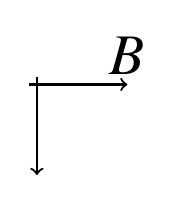
\begin{tikzpicture}
      \draw[->,thick] (-.1,0)--(1.15,0) node[above]
        {\huge $B$};
        % {Number of behaviors $B$};
      \draw[->,thick] (0,.1)--(0,-1.15) node[below]
        {\huge $\pilow$};
        % {Low payoff frequency $\pilow$};
	  \end{tikzpicture}~\\[-2em]

    \begin{minipage}{3.75in}
      \centering
      {\hspace{5.25em}\huge $B = 2$}
    \end{minipage}%
    \begin{minipage}{3.75in}
      \centering
      {\hspace{1.0em}\huge $B = 4$}
    \end{minipage}%
    \begin{minipage}{3.75in}
      \centering
      {\hspace{2.0em}\huge $B = 10$}
    \end{minipage}~\\

    \begin{minipage}{3.75in}
    \begin{rotate}{90}
      {\parbox{2.5in}{
          \centering
          \vspace{-2.5em} {\huge$ \pilow = 0.1$} \\
          {\begin{rotate}{-90}{\huge $\meansl$}\hspace{3em}\end{rotate}}
      }}
    \end{rotate}%
    \hspace{2em}
      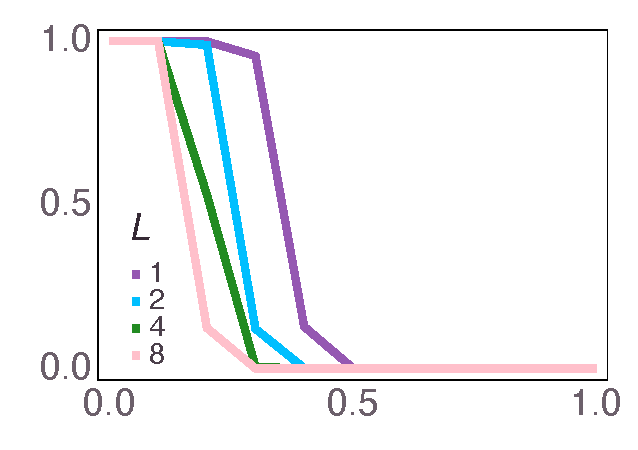
\includegraphics[width=\textwidth]{mean_social_learner_over_u_lowpayoff=0.1_nbehaviors=2.pdf}
    \end{minipage}\noindent\hspace{1.25em}
	\begin{minipage}{3.75in}%
      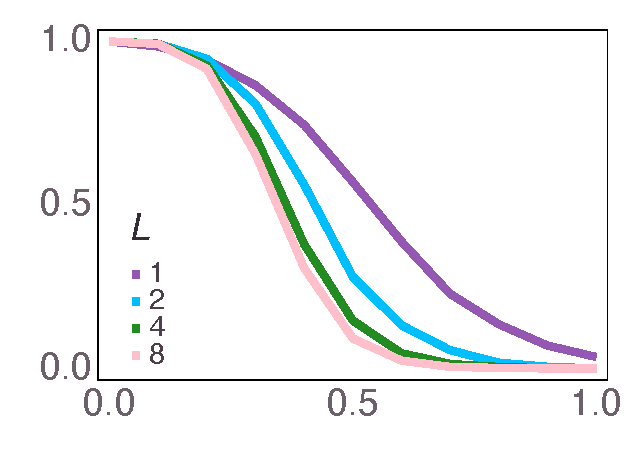
\includegraphics[width=\textwidth]{mean_social_learner_over_u_lowpayoff=0.1_nbehaviors=4.pdf}
    \end{minipage}\noindent
	\begin{minipage}{3.75in}%
      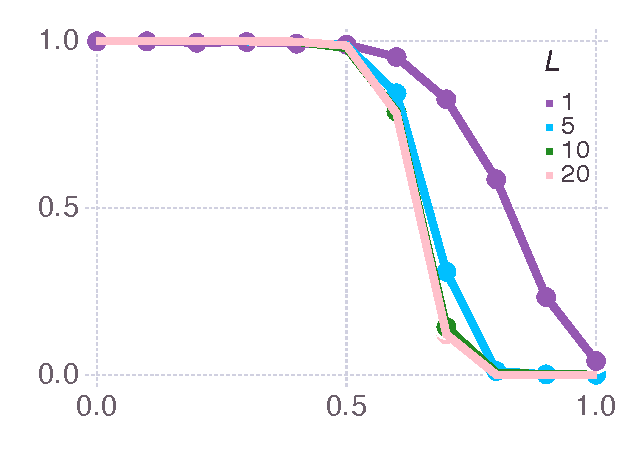
\includegraphics[width=\textwidth]{mean_social_learner_over_u_lowpayoff=0.1_nbehaviors=10.pdf}
    \end{minipage}~\\[0.5em]

    \begin{minipage}{3.75in}
    \begin{rotate}{90}
      {\parbox{2.5in}{
          \centering
          \vspace{-2.5em} {\huge$ \pilow = 0.45$} \\
          {\begin{rotate}{-90}{\huge $\meansl$}\hspace{3em}\end{rotate}}
      }}
    \end{rotate}%
    \hspace{2em}
      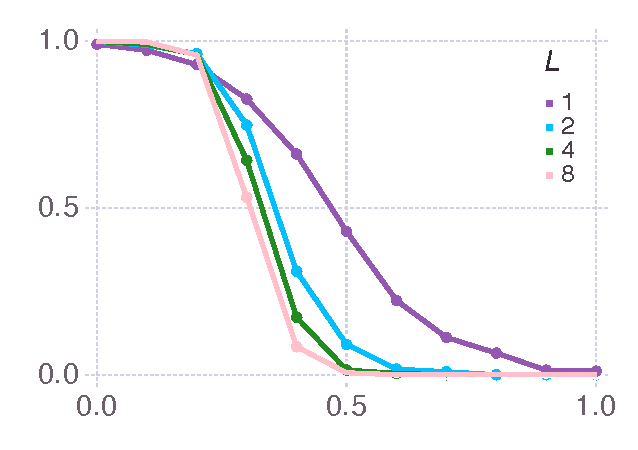
\includegraphics[width=\textwidth]{mean_social_learner_over_u_lowpayoff=0.45_nbehaviors=2.pdf}
	\end{minipage}\noindent\hspace{1.25em}
	\begin{minipage}{3.75in}%
      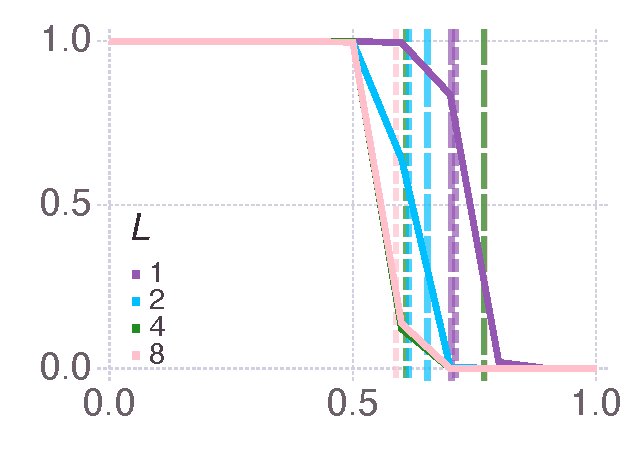
\includegraphics[width=\textwidth]{mean_social_learner_over_u_lowpayoff=0.45_nbehaviors=4.pdf}
    \end{minipage}\noindent
	\begin{minipage}{3.75in}%
      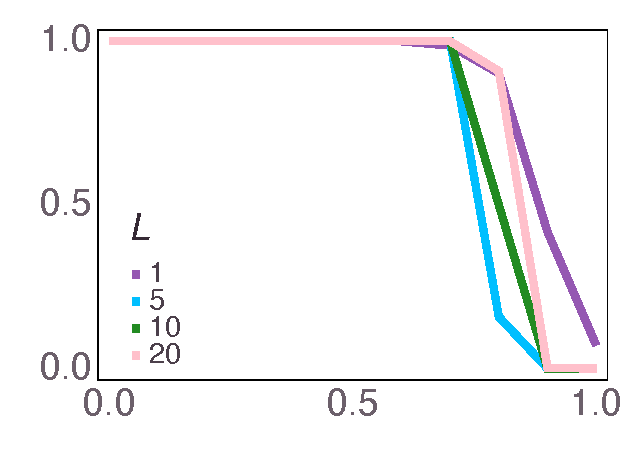
\includegraphics[width=\textwidth]{mean_social_learner_over_u_lowpayoff=0.45_nbehaviors=10.pdf}
    \end{minipage}~\\[0.5em]

    \begin{minipage}{3.75in}
    \begin{rotate}{90}
      {\parbox{2.5in}{
          \centering
          \vspace{-2.5em} {\huge$ \pilow = 0.8$} \\
          {\begin{rotate}{-90}{\huge $\meansl$}\hspace{3em}\end{rotate}}
      }}
    \end{rotate}%
    \hspace{2em}
      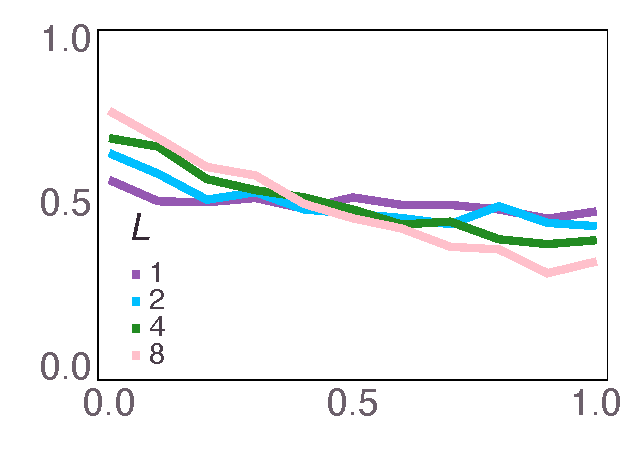
\includegraphics[width=\textwidth]{mean_social_learner_over_u_lowpayoff=0.8_nbehaviors=2.pdf}
        \\[-2.75em]
        \begin{center}
          {\hspace{3.25em} \huge $\quad u$}
      \end{center}
	  \end{minipage}\noindent\hspace{1.25em}
		\begin{minipage}{3.75in}%
		  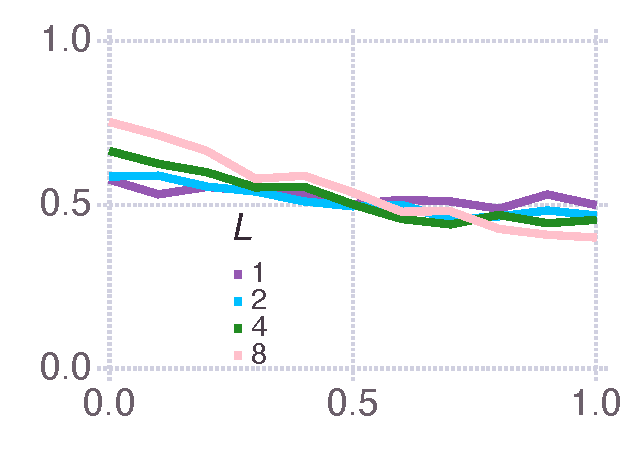
\includegraphics[width=\textwidth]{mean_social_learner_over_u_lowpayoff=0.8_nbehaviors=4.pdf}
		  \\[-2.75em]
	  \begin{center}
        {\huge $\quad u$}
      \end{center}
    \end{minipage}
	\begin{minipage}{3.75in}%
		  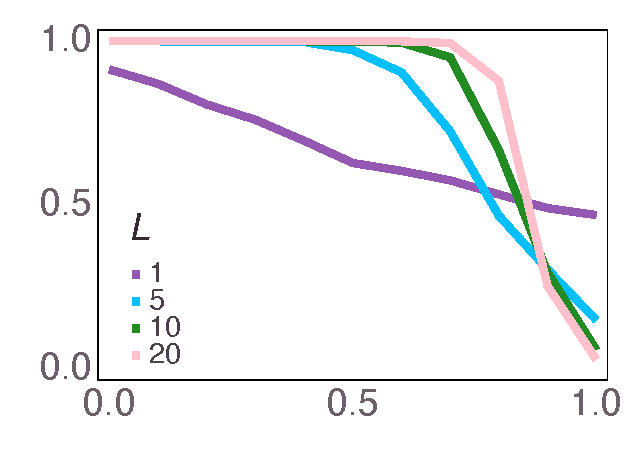
\includegraphics[width=\textwidth]{mean_social_learner_over_u_lowpayoff=0.8_nbehaviors=10.pdf}
		  \\[-2.75em]
	  \begin{center}
        {\huge $\quad u$}
      \end{center}
	\end{minipage}%
\end{document}


\documentclass[varwidth=true,crop=false]{standalone}
\usepackage[chatter]{rotating}
\usepackage{amssymb,amsmath}
\usepackage{pgfplots}

\usepackage{geometry}
\geometry{
paperwidth=12in,
paperheight=12in,
margin=0.25in
}

\newcommand{\pisub}[1]{\pi_{\mathrm{#1}}}
\newcommand{\pilow}{\pisub{low}}
\newcommand{\pihigh}{\pisub{high}}
\newcommand{\piI}{\langle \pisub{I} \rangle}
\newcommand{\piS}{\langle \pisub{S} \rangle}
\newcommand{\ledger}{\bar\pi_{ib}}

\newcommand{\meanvar}[1]{\langle #1 \rangle}
\newcommand{\meansl}{\meanvar{s}}
\newcommand{\meanpi}{\meanvar{\pi}}
\newcommand{\meansoc}{\meanvar{\pi_\mathrm{S}}}
\newcommand{\meanasoc}{\meanvar{\pi_\mathrm{A}}}
\newcommand{\meanT}{\meanvar{T}}

\newcommand{\bandit}{\text{Bandit}_b(0, 1)}

\begin{document}
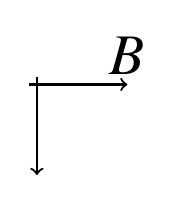
\begin{tikzpicture}
      \draw[->,thick] (-.1,0)--(1.15,0) node[above]
        {\huge $B$};
        % {Number of behaviors $B$};
      \draw[->,thick] (0,.1)--(0,-1.15) node[below]
        {\huge $\pilow$};
        % {Low payoff frequency $\pilow$};
	  \end{tikzpicture}~\\[-2em]

    \begin{minipage}{3.75in}
      \centering
      {\hspace{5.25em}\huge $B = 2$}
    \end{minipage}%
    \begin{minipage}{3.75in}
      \centering
      {\hspace{1.0em}\huge $B = 4$}
    \end{minipage}%
    \begin{minipage}{3.75in}
      \centering
      {\hspace{2.0em}\huge $B = 10$}
    \end{minipage}~\\

    \begin{minipage}{3.75in}
    \begin{rotate}{90}
      {\parbox{2.5in}{
          \centering
          \vspace{-2.5em} {\huge$ \pilow = 0.1$} \\
          {\begin{rotate}{-90}{\huge $\frac{\meanpi}{L}$}\hspace{3em}\end{rotate}}
      }}
    \end{rotate}%
    \hspace{2em}
      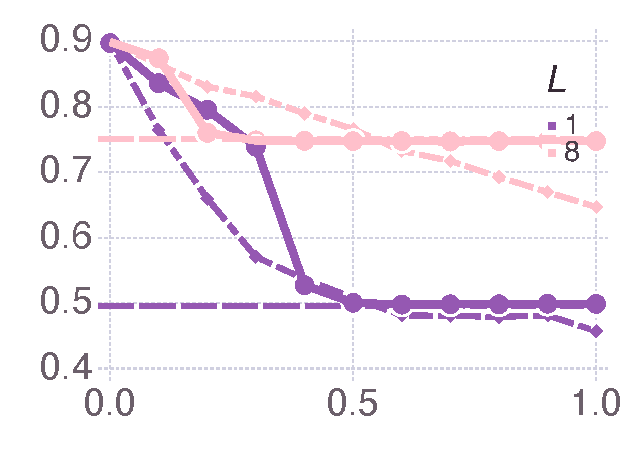
\includegraphics[width=\textwidth]{Figures/mean_prev_net_payoff_over_u_lowpayoff=0.1_nbehaviors=2.pdf}
    \end{minipage}\noindent\hspace{1.25em}
	\begin{minipage}{3.75in}%
      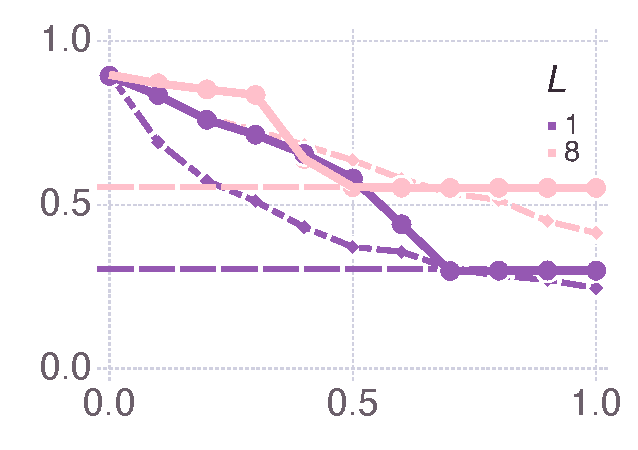
\includegraphics[width=\textwidth]{Figures/mean_prev_net_payoff_over_u_lowpayoff=0.1_nbehaviors=4.pdf}
    \end{minipage}\noindent
	\begin{minipage}{3.75in}%
      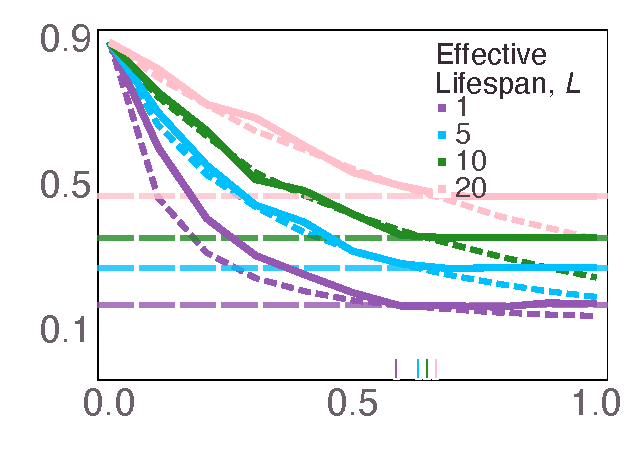
\includegraphics[width=\textwidth]{Figures/mean_prev_net_payoff_over_u_lowpayoff=0.1_nbehaviors=10.pdf}
    \end{minipage}~\\[0.5em]

    \begin{minipage}{3.75in}
    \begin{rotate}{90}
      {\parbox{2.5in}{
          \centering
          \vspace{-2.5em} {\huge$ \pilow = 0.45$} \\
          {\begin{rotate}{-90}{\huge $\frac{\meanpi}{L}$}\hspace{3em}\end{rotate}}
      }}
    \end{rotate}%
    \hspace{2em}
      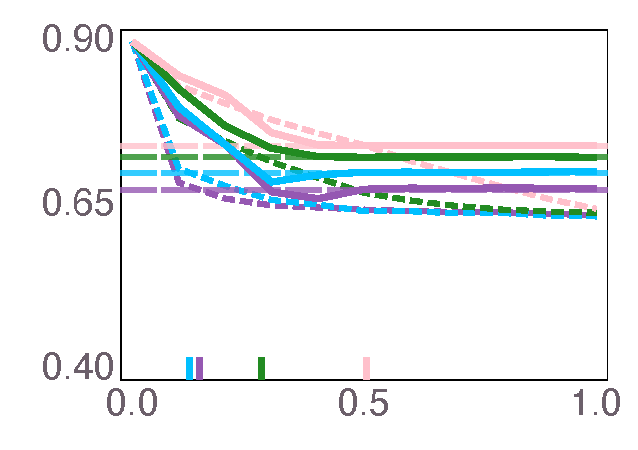
\includegraphics[width=\textwidth]{Figures/mean_prev_net_payoff_over_u_lowpayoff=0.45_nbehaviors=2.pdf}
	\end{minipage}\noindent\hspace{1.25em}
	\begin{minipage}{3.75in}%
      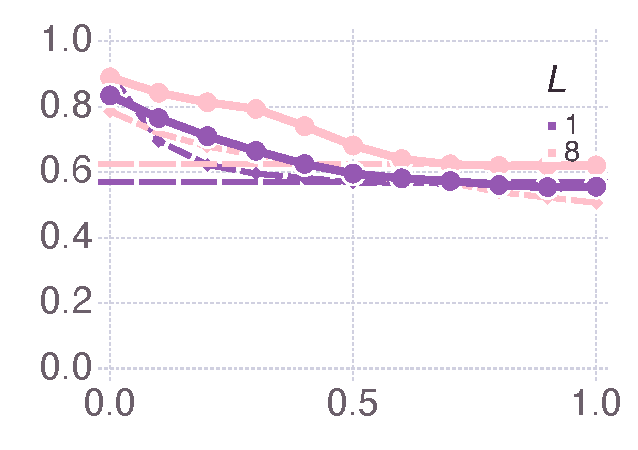
\includegraphics[width=\textwidth]{Figures/mean_prev_net_payoff_over_u_lowpayoff=0.45_nbehaviors=4.pdf}
    \end{minipage}\noindent
	\begin{minipage}{3.75in}%
      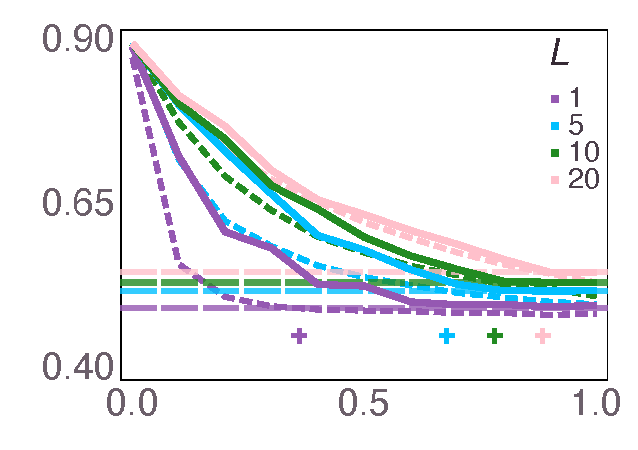
\includegraphics[width=\textwidth]{Figures/mean_prev_net_payoff_over_u_lowpayoff=0.45_nbehaviors=10.pdf}
    \end{minipage}~\\[0.5em]

    \begin{minipage}{3.75in}
    \begin{rotate}{90}
      {\parbox{2.5in}{
          \centering
          \vspace{-2.5em} {\huge$ \pilow = 0.8$} \\
          {\begin{rotate}{-90}{\huge $\frac{\meanpi}{L}$}\hspace{3em}\end{rotate}}
      }}
    \end{rotate}%
    \hspace{2em}
      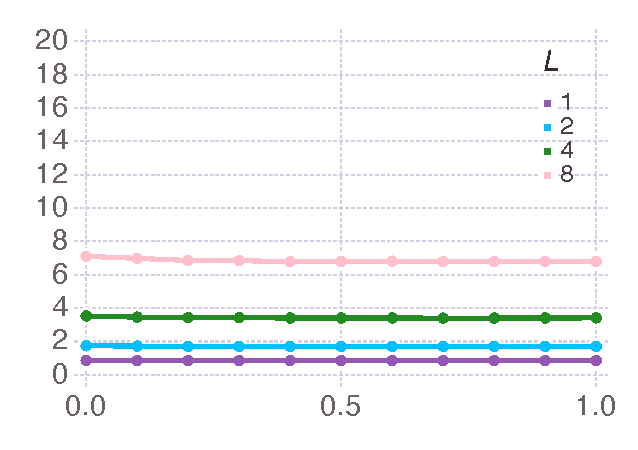
\includegraphics[width=\textwidth]{Figures/mean_prev_net_payoff_over_u_lowpayoff=0.8_nbehaviors=2.pdf}
        \\[-2.75em]
        \begin{center}
          {\hspace{3.25em} \huge $\quad u$}
      \end{center}
	  \end{minipage}\noindent\hspace{1.25em}
		\begin{minipage}{3.75in}%
		  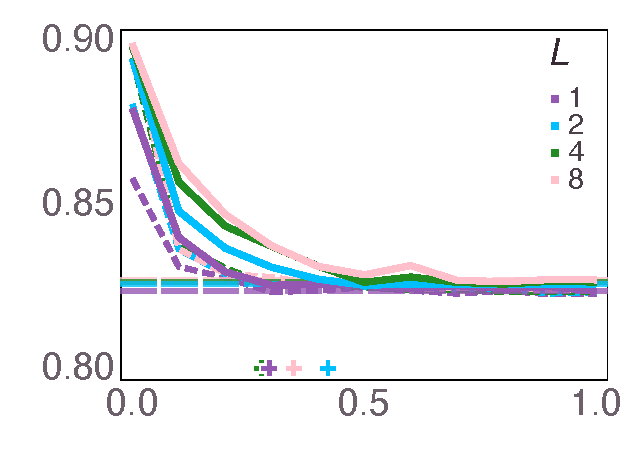
\includegraphics[width=\textwidth]{Figures/mean_prev_net_payoff_over_u_lowpayoff=0.8_nbehaviors=4.pdf}
		  \\[-2.75em]
	  \begin{center}
        {\huge $\quad u$}
      \end{center}
    \end{minipage}
	\begin{minipage}{3.75in}%
		  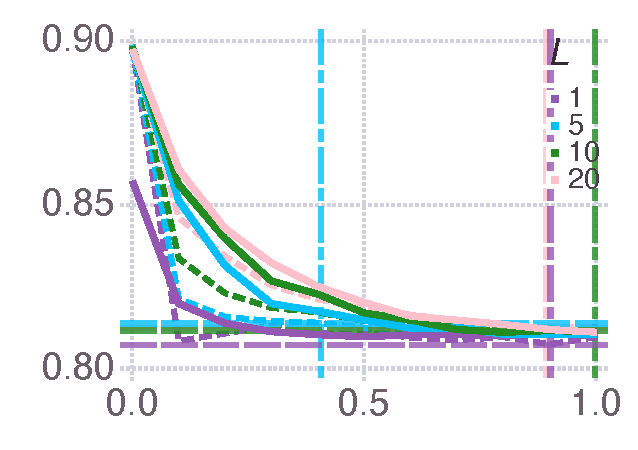
\includegraphics[width=\textwidth]{Figures/mean_prev_net_payoff_over_u_lowpayoff=0.8_nbehaviors=10.pdf}
		  \\[-2.75em]
	  \begin{center}
        {\huge $\quad u$}
      \end{center}
    \end{minipage} \\[2.5em]

    \begin{center}
       
\includegraphics[width=1.85in]{Figures/legendElements/dot.pdf}
       {\huge Average all-social population payoffs}  \\[1.125em]
       
\includegraphics[width=1.85in]{Figures/legendElements/ldash.pdf} 
       {\huge Average all-asocial population payoffs} \\[1.125em]
       
\includegraphics[width=1.85in]{Figures/legendElements/solid.pdf} 
       {\huge Simulated average population payoffs} \\[1.125em]
      {\Huge \textbf{+} \huge $u$ value where homogenous social and asocial payoffs
      are equal} 
    \end{center}

\end{document}


\documentclass[varwidth=true,crop=false]{standalone}
\usepackage[chatter]{rotating}
\usepackage{amssymb,amsmath}
\usepackage{pgfplots}

\usepackage{geometry}
\geometry{
paperwidth=8in,
paperheight=6.25in,
margin=0.25in
}

\newcommand{\pisub}[1]{\pi_{\mathrm{#1}}}
\newcommand{\pilow}{\pisub{low}}
\newcommand{\pihigh}{\pisub{high}}
\newcommand{\piI}{\langle \pisub{I} \rangle}
\newcommand{\piS}{\langle \pisub{S} \rangle}
\newcommand{\ledger}{\bar\pi_{ib}}

\newcommand{\meanvar}[1]{\langle #1 \rangle}
\newcommand{\meansl}{\meanvar{s}}
\newcommand{\meanpi}{\meanvar{\pi}}
\newcommand{\meansoc}{\meanvar{\pi_\mathrm{S}}}
\newcommand{\meanasoc}{\meanvar{\pi_\mathrm{A}}}
\newcommand{\meanT}{\meanvar{T}}

\newcommand{\bandit}{\text{Bandit}_b(0, 1)}

\begin{document}

    \begin{minipage}{3.75in}
      \centering
      {\hspace{5.25em}\huge $B = 4$}
    \end{minipage}%
    \begin{minipage}{3.75in}
      \centering
      {\hspace{2.0em}\huge $B = 10$}
    \end{minipage}~\\

    \begin{minipage}{3.75in}
    \begin{rotate}{90}
      {\parbox{2.5in}{
          \centering
          \vspace{-2.5em} {\huge$ \pilow = 0.1$} \\
          {\begin{rotate}{-90}{\huge $\frac{\meanT}{L}$}\hspace{3em}\end{rotate}}
      }}
    \end{rotate}%
    \hspace{2em}
      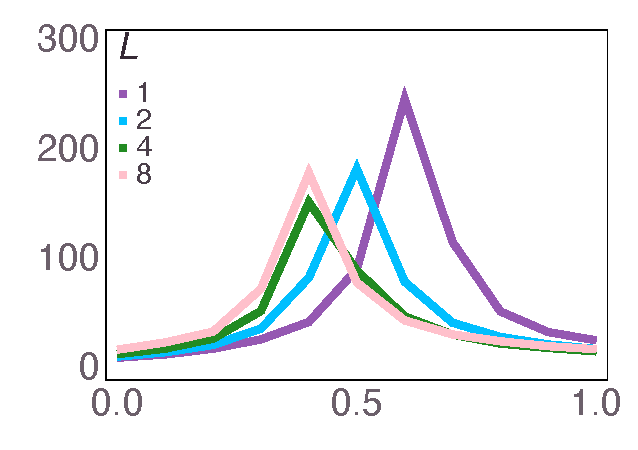
\includegraphics[width=\textwidth]{Figures/step_over_u_lowpayoff=0.1_nbehaviors=4.pdf}
    \end{minipage}\noindent\begin{minipage}{3.75in}%
      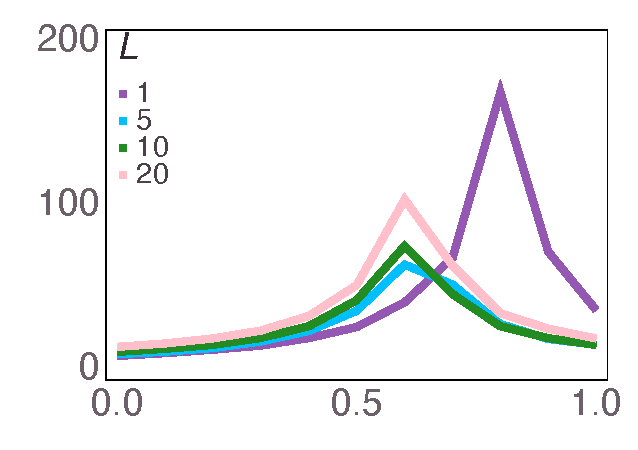
\includegraphics[width=\textwidth]{Figures/step_over_u_lowpayoff=0.1_nbehaviors=10.pdf}
    \end{minipage}~\\[0.5em]

    \begin{minipage}{3.75in}
    \begin{rotate}{90}
      {\parbox{2.5in}{
          \centering
          \vspace{-2.5em} {\huge$ \pilow = 0.45$} \\
          {\begin{rotate}{-90}{\huge $\frac{\meanT}{L}$}\hspace{3em}\end{rotate}}
      }}
    \end{rotate}%
    \hspace{2em}
      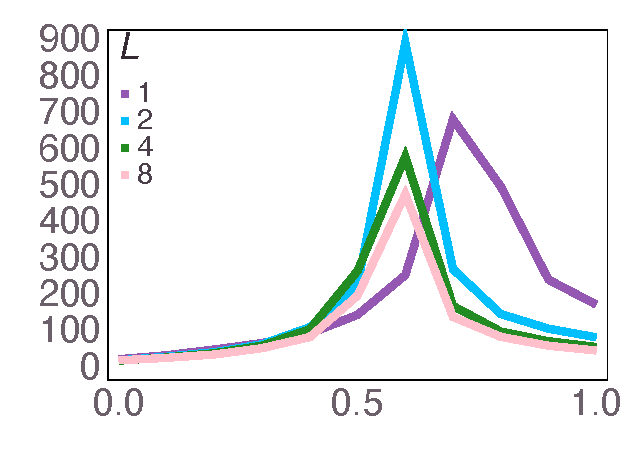
\includegraphics[width=\textwidth]{Figures/step_over_u_lowpayoff=0.45_nbehaviors=4.pdf}
        \\[-2.75em]
        \begin{center}
          {\hspace{3.25em} \huge $\quad u$}
      \end{center}
        \end{minipage}\noindent\begin{minipage}{3.75in}%
      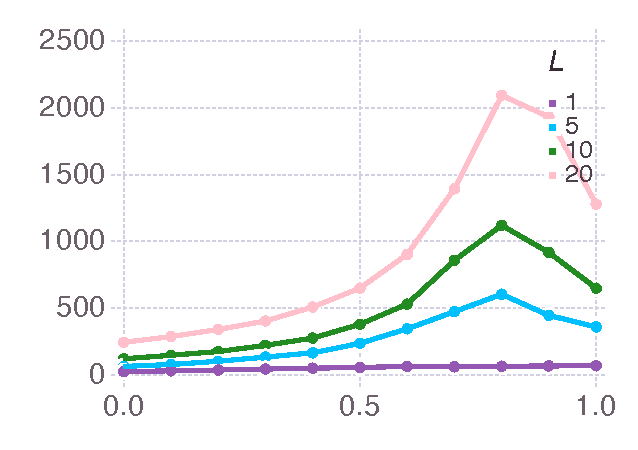
\includegraphics[width=\textwidth]{Figures/step_over_u_lowpayoff=0.45_nbehaviors=10.pdf}
      \\[-2.75em]
      \begin{center}
        {\huge $\quad u$}
      \end{center}
    \end{minipage}
\end{document}

=======
The shape of the decrease from all agents
always becoming social learners ($\meansl = 1.0$) to 
all agents always becoming individual learners ($\meansl = 0.0$)
is heterogeneous. We identified patterns in this heterogeneity that inform our
understanding of when and how social learning is advantageous, and when 
and why individual learning is advantageous. 
Changes in the uncertainty parameters ($\pilow$, $B$, $L$) 
result in the following changes in the shape of the transition from $\meansl = 1.0$ 
to $\meansl = 0.0$: (1) the transition
occurs at different critical values of $u$; and (2) the transition occurs
with greater or lesser rapidity over $u$. 
For instance, when $B=2$, $\pilow = 0.1$, and $L=8$, $\meansl$ goes from 1 to 
0 starting at $u=0.1$ and reaches 0 at $u=0.3$ (Figure~\ref{fig:evolutionOfSL},
top left). When we increased $B=4$ (Figure~\ref{fig:evolutionOfSL}, top center), the
transition from $\meansl = 1$ to 0 begins at $u=0.3$. When $B=4$, $\pilow=0.1$,
and $L=1$ the transition from $\meansl=1$ to 0 begins at $u=0.3$ but does not
reach 0 until $u \approx 0.9$ (again Figure~\ref{fig:evolutionOfSL}, top center).

We can draw some conclusions about the evolution of social learning by analyzing the
location and shape of the suppression of social learning as $u$ was increased.
First, let us observe some general trends. Increased $\pilow$ generally
flattened the suppression of social learning as $u$ increased.  
Increased $B$ tended to increase the critical value of $u$ at which the 
system transitions from favoring social learning to favor individual learning.  
Increased $L$ generally sharpened the suppression of social learning.
Within each of these broad trends over the uncertainty parameters are several
details that depend on context as defined by the values of the other uncertainty
parameters.

When $\pilow$ was increased, the suppression of social learning was, in
general, less rapid as $u$ increased. This effect is particularly acute when
$\pilow = 0.8$, which is very nearly equal to the expected value of the optimal
payoff, $\pihigh = 0.9$. When $\pilow = 0.8$ $\meansl$ never actually reaches 
1 or 0 for any parameter settings. The suppression of social learning in this
case is approximately linear, if there is selection at all. When $\pilow = 0.8$
and $L = 1$ there is little to no selection across $B$, 
so populations evolve randomly towards $\meansl = 1$ or $\meansl = 0$. 

Increased $B$ generally led to increased critical $u$ at which social learning
starts to be suppresed. When payoffs are not ambiguous ($\pilow = 0.1$), the the
suppression of social learning starts at $u \approx 0.1$ for $B=2$; at $u \approx
0.3$ when $B=4$; and at $u \approx 0.5$ when $B=10$.  When payoffs are more
ambiguous ($\pilow = 0.45,0.8$), increased $B$ also led to a flattening of the
suppression of social learning when $L=1$. 

The general effect of $L$ is to increase the rapidity of the suppression of social
learning via the strengthening of selection pressure since longer-lived agents
build up stronger priors over their lifetimes. If it is advantageous to
learn socially, this will be reliably detected. Inversely, decreased $L$
can weaken selection pressure since agents cannot amass useful information when
$L$ is small. This is most extreme when $\pilow = 0.8$ and there is little to
no selection for or against social learning when $L=1$. However, decreased $L$ can
also delay the suppression of social learning as $u$ increases, since social
learning provdes agents with the possibility of learning what the optimal behavior
might be.  Even when $u$ was large, agents with a lifespan of 1 more often evolved
to be social learners because social learning was to be preferred over random
chance.


\subsection{Social learning capacity increases payoffs}

For social learning to reliably evolve, it must be more beneficial
(in terms of payoffs) than individual learning. Inversely, social learning
should be suppressed when it misleads agents away from quickly identifying the
optimal behavior through individual learning.
We found that different parameter settings indeed change how 
advantageous social learning
is compared to individual learning (Figure~\ref{fig:meanNetPayoffs}).
We find that the transition from $\meansl = 1$ to $\meansl = 0$ occurs when
the mean net payoff among populations of all social learners is close to 
that of the expected individual learner payoff, $\piI$.

To analyze the effect of uncertainty on
payoffs, it is useful to identify some constant reference values which we will
use to evaluate the benefit of social learning. First, the optimal expected payoff
is the optimal behavior payoff times the lifespan, which we can denote
$\langle \pi^*(L) \rangle = L\cdot\pihigh$. The expected base payoff by chance is 
$\langle \pi_{\text{base}} \rangle = L \left[ (B - 1) \pilow + \pihigh \right]$, which
an agent would receive on average from performing purely random behaviors. 
Most importantly for understanding the benefit and evolution of social learning,
we calculated by simulation the expected payoff to individual learners for
each triplet ($\pilow$, $B$, $L$), which we denote $\piI$
and plot for reference in Figure~\ref{fig:meanNetPayoffs}. Note 
$\piI$ is insensitive to $u$, which only affects the benefit of social
learning.

We observe across parameter settings that social learning outperforms
individual learning when $u$ is small. In fact, when $u=0.0$, social learning
enables each new generation to know the optimal behavior and achieve the
maximum expected payoff for their lifespan, $\langle \pi^*(L) \rangle$.
However, in some cases, even when $u$ is small, the returns on social learning
are truly marginal due to relatively high, uniform expected payoffs whether or
not agents identify the optimal behavior, especially when $\pilow = 0.8$. In
intermediate cases, examining the decay of the benefit of social learning
informs our understanding of social learning evolution analyzed above.  

As our analysis of social learning evolution suggested, social learning is only
beneficial up to a point. When $\pilow=0.1$, increased $B$ led both to larger
differences between payoffs when social learning was more beneficial, and it
led to $\piS > \piI$ across more values of $u$. This occurs because when there
are fewer behaviors it is easier for non-social learners to identify the
optimal behavior on their own. Even relatively small values of $u$ disrupt
the fidelity of social learning to the point that it being misled is
prohibitively costly compared to simply finding the optimal on one's own.
A relatively short lifespan can also extend the utility of social learning
across more values of $u$ since there are fewer opportunities for agents to
independently identify and perform the optimal solution. 

\subsection{Evolutionary outcome uncertainty} 

Finally, we found that the \emph{evolutionary uncertainty} of the system
increases around the values of $u$ where $\meansl$ goes from 1 to 0.  We know
that outcomes are uncertain in this region because we know that $\meansl$
is equivalent to the fraction of outcomes that ended with all agents being
social learners. $1 - \meansl$ is the fraction of trials that ended with 
all agents becoming individual learners. Therefore, when $\meansl \approx 0.5$,
this means roughly half of the simulated trials fixated at $\meansl = 1.0$
while the other half fixated at $\meansl = 0.0$.
Only 44 of nearly 400k trials did not go to fixation ($\meansl = 1$ or $\meansl = 0$) 
within 20k maximum iterations (Table~\ref{tab:convergence}); all that did not
reach fixation had $B=10$. 

We also measured environmental uncertainty more directly, in terms of the
expected number of time steps to convergence, $\langle T \rangle$.
Evolutionary uncertainty is thus an outcome measure---an emergent form of
uncertainty due to weak selection pressures. We found that increased $\pilow$
tended to increase the overall uncertainty in terms of $\langle T \rangle$.
Increasing $B$ also increased the $u$ at which $\langle T \rangle$ peaked.
This indicates the evolutionary system is significantly less certain of 
which behavior is optimal around critical uncertainty parameter ensembles.

\mt{interpret this further}



\documentclass[varwidth=true,crop=false]{standalone}
\usepackage[chatter]{rotating}
\usepackage{amssymb,amsmath}
\usepackage{pgfplots}

\usepackage{geometry}
\geometry{
paperwidth=12in,
paperheight=12in,
margin=0.25in
}

\newcommand{\pisub}[1]{\pi_{\mathrm{#1}}}
\newcommand{\pilow}{\pisub{low}}
\newcommand{\pihigh}{\pisub{high}}
\newcommand{\piI}{\langle \pisub{I} \rangle}
\newcommand{\piS}{\langle \pisub{S} \rangle}
\newcommand{\ledger}{\bar\pi_{ib}}

\newcommand{\meanvar}[1]{\langle #1 \rangle}
\newcommand{\meansl}{\meanvar{s}}
\newcommand{\meanpi}{\meanvar{\pi}}
\newcommand{\meansoc}{\meanvar{\pi_\mathrm{S}}}
\newcommand{\meanasoc}{\meanvar{\pi_\mathrm{A}}}
\newcommand{\meanT}{\meanvar{T}}

\newcommand{\bandit}{\text{Bandit}_b(0, 1)}

\begin{document}
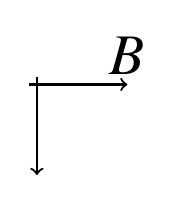
\begin{tikzpicture}
      \draw[->,thick] (-.1,0)--(1.15,0) node[above]
        {\huge $B$};
        % {Number of behaviors $B$};
      \draw[->,thick] (0,.1)--(0,-1.15) node[below]
        {\huge $\pilow$};
        % {Low payoff frequency $\pilow$};
	  \end{tikzpicture}~\\[-2em]

    \begin{minipage}{3.75in}
      \centering
      {\hspace{5.25em}\huge $B = 2$}
    \end{minipage}%
    \begin{minipage}{3.75in}
      \centering
      {\hspace{1.0em}\huge $B = 4$}
    \end{minipage}%
    \begin{minipage}{3.75in}
      \centering
      {\hspace{2.0em}\huge $B = 10$}
    \end{minipage}~\\

    \begin{minipage}{3.75in}
    \begin{rotate}{90}
      {\parbox{2.5in}{
          \centering
          \vspace{-2.5em} {\huge$ \pilow = 0.1$} \\
          {\begin{rotate}{-90}{\huge $\meansl$}\hspace{3em}\end{rotate}}
      }}
    \end{rotate}%
    \hspace{2em}
      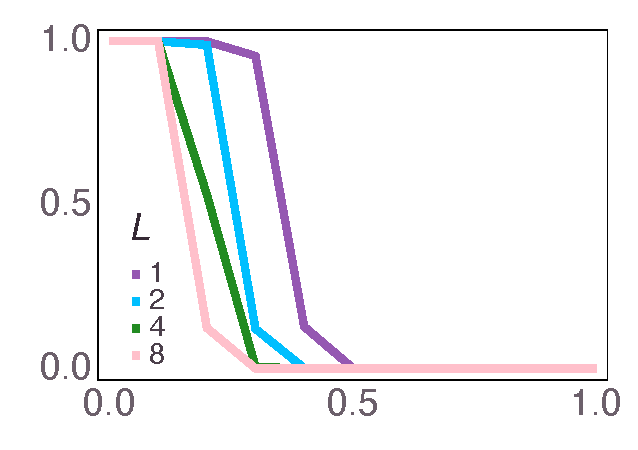
\includegraphics[width=\textwidth]{mean_social_learner_over_u_lowpayoff=0.1_nbehaviors=2.pdf}
    \end{minipage}\noindent\hspace{1.25em}
	\begin{minipage}{3.75in}%
      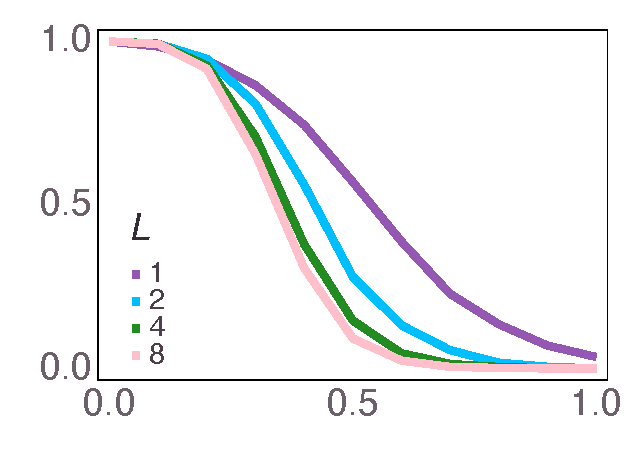
\includegraphics[width=\textwidth]{mean_social_learner_over_u_lowpayoff=0.1_nbehaviors=4.pdf}
    \end{minipage}\noindent
	\begin{minipage}{3.75in}%
      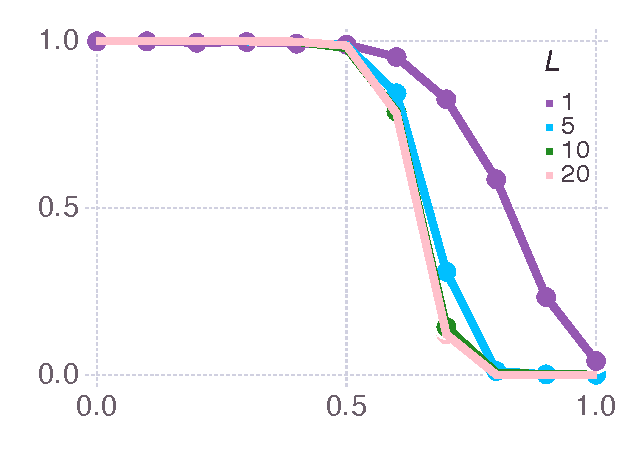
\includegraphics[width=\textwidth]{mean_social_learner_over_u_lowpayoff=0.1_nbehaviors=10.pdf}
    \end{minipage}~\\[0.5em]

    \begin{minipage}{3.75in}
    \begin{rotate}{90}
      {\parbox{2.5in}{
          \centering
          \vspace{-2.5em} {\huge$ \pilow = 0.45$} \\
          {\begin{rotate}{-90}{\huge $\meansl$}\hspace{3em}\end{rotate}}
      }}
    \end{rotate}%
    \hspace{2em}
      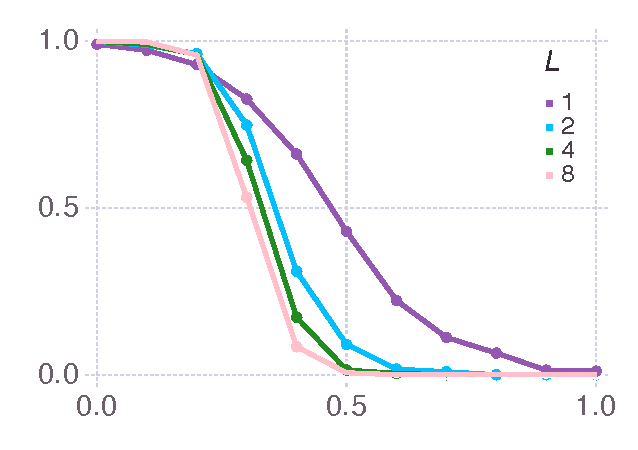
\includegraphics[width=\textwidth]{mean_social_learner_over_u_lowpayoff=0.45_nbehaviors=2.pdf}
	\end{minipage}\noindent\hspace{1.25em}
	\begin{minipage}{3.75in}%
      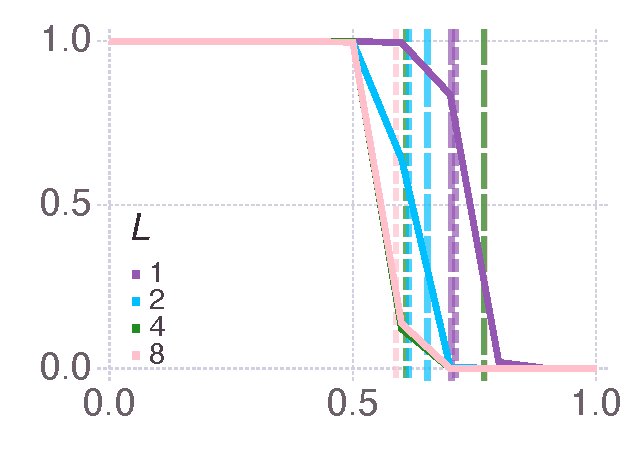
\includegraphics[width=\textwidth]{mean_social_learner_over_u_lowpayoff=0.45_nbehaviors=4.pdf}
    \end{minipage}\noindent
	\begin{minipage}{3.75in}%
      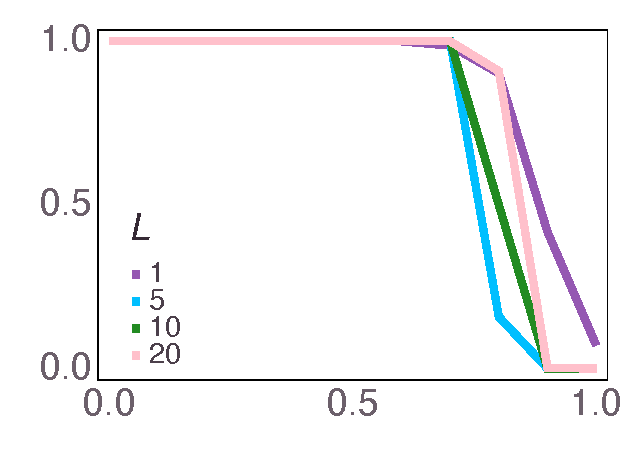
\includegraphics[width=\textwidth]{mean_social_learner_over_u_lowpayoff=0.45_nbehaviors=10.pdf}
    \end{minipage}~\\[0.5em]

    \begin{minipage}{3.75in}
    \begin{rotate}{90}
      {\parbox{2.5in}{
          \centering
          \vspace{-2.5em} {\huge$ \pilow = 0.8$} \\
          {\begin{rotate}{-90}{\huge $\meansl$}\hspace{3em}\end{rotate}}
      }}
    \end{rotate}%
    \hspace{2em}
      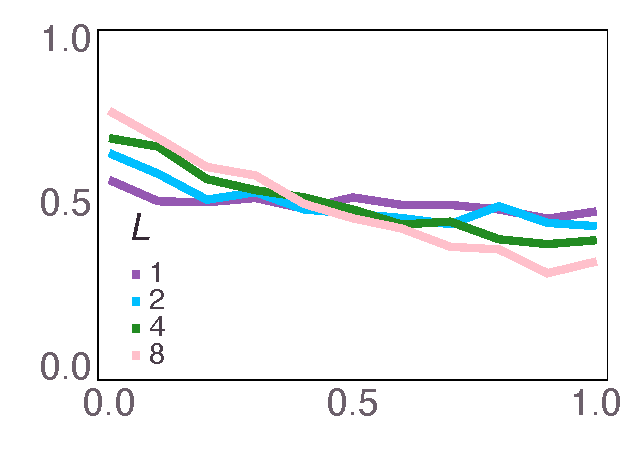
\includegraphics[width=\textwidth]{mean_social_learner_over_u_lowpayoff=0.8_nbehaviors=2.pdf}
        \\[-2.75em]
        \begin{center}
          {\hspace{3.25em} \huge $\quad u$}
      \end{center}
	  \end{minipage}\noindent\hspace{1.25em}
		\begin{minipage}{3.75in}%
		  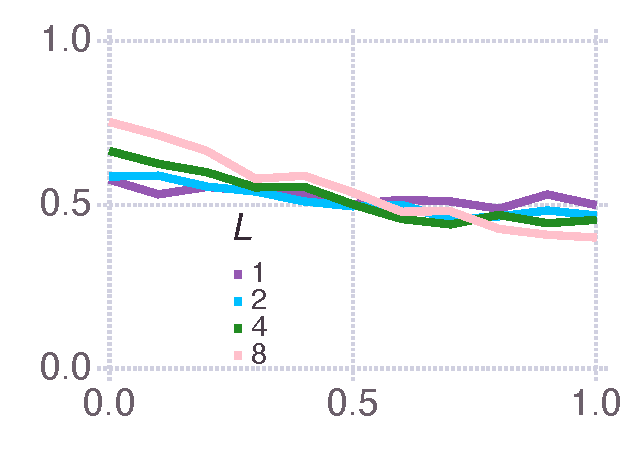
\includegraphics[width=\textwidth]{mean_social_learner_over_u_lowpayoff=0.8_nbehaviors=4.pdf}
		  \\[-2.75em]
	  \begin{center}
        {\huge $\quad u$}
      \end{center}
    \end{minipage}
	\begin{minipage}{3.75in}%
		  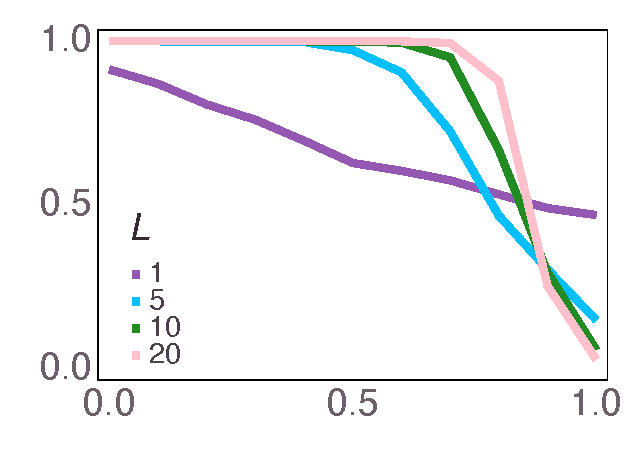
\includegraphics[width=\textwidth]{mean_social_learner_over_u_lowpayoff=0.8_nbehaviors=10.pdf}
		  \\[-2.75em]
	  \begin{center}
        {\huge $\quad u$}
      \end{center}
	\end{minipage}%
\end{document}


\documentclass[varwidth=true,crop=false]{standalone}
\usepackage[chatter]{rotating}
\usepackage{amssymb,amsmath}
\usepackage{pgfplots}

\usepackage{geometry}
\geometry{
paperwidth=12in,
paperheight=12in,
margin=0.25in
}

\newcommand{\pisub}[1]{\pi_{\mathrm{#1}}}
\newcommand{\pilow}{\pisub{low}}
\newcommand{\pihigh}{\pisub{high}}
\newcommand{\piI}{\langle \pisub{I} \rangle}
\newcommand{\piS}{\langle \pisub{S} \rangle}
\newcommand{\ledger}{\bar\pi_{ib}}

\newcommand{\meanvar}[1]{\langle #1 \rangle}
\newcommand{\meansl}{\meanvar{s}}
\newcommand{\meanpi}{\meanvar{\pi}}
\newcommand{\meansoc}{\meanvar{\pi_\mathrm{S}}}
\newcommand{\meanasoc}{\meanvar{\pi_\mathrm{A}}}
\newcommand{\meanT}{\meanvar{T}}

\newcommand{\bandit}{\text{Bandit}_b(0, 1)}

\begin{document}
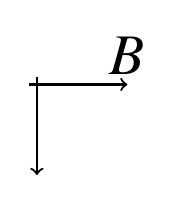
\begin{tikzpicture}
      \draw[->,thick] (-.1,0)--(1.15,0) node[above]
        {\huge $B$};
        % {Number of behaviors $B$};
      \draw[->,thick] (0,.1)--(0,-1.15) node[below]
        {\huge $\pilow$};
        % {Low payoff frequency $\pilow$};
	  \end{tikzpicture}~\\[-2em]

    \begin{minipage}{3.75in}
      \centering
      {\hspace{5.25em}\huge $B = 2$}
    \end{minipage}%
    \begin{minipage}{3.75in}
      \centering
      {\hspace{1.0em}\huge $B = 4$}
    \end{minipage}%
    \begin{minipage}{3.75in}
      \centering
      {\hspace{2.0em}\huge $B = 10$}
    \end{minipage}~\\

    \begin{minipage}{3.75in}
    \begin{rotate}{90}
      {\parbox{2.5in}{
          \centering
          \vspace{-2.5em} {\huge$ \pilow = 0.1$} \\
          {\begin{rotate}{-90}{\huge $\frac{\meanpi}{L}$}\hspace{3em}\end{rotate}}
      }}
    \end{rotate}%
    \hspace{2em}
      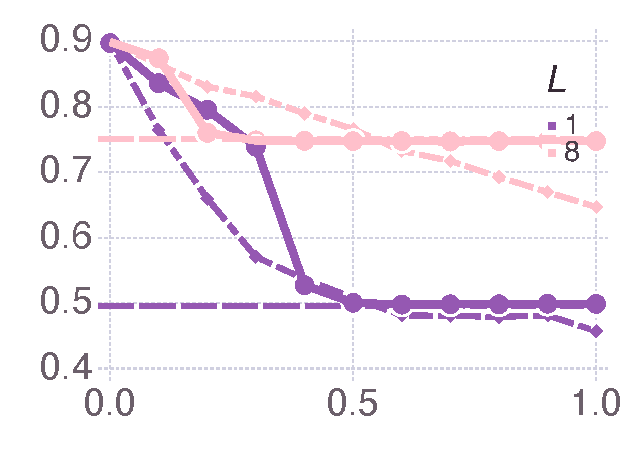
\includegraphics[width=\textwidth]{Figures/mean_prev_net_payoff_over_u_lowpayoff=0.1_nbehaviors=2.pdf}
    \end{minipage}\noindent\hspace{1.25em}
	\begin{minipage}{3.75in}%
      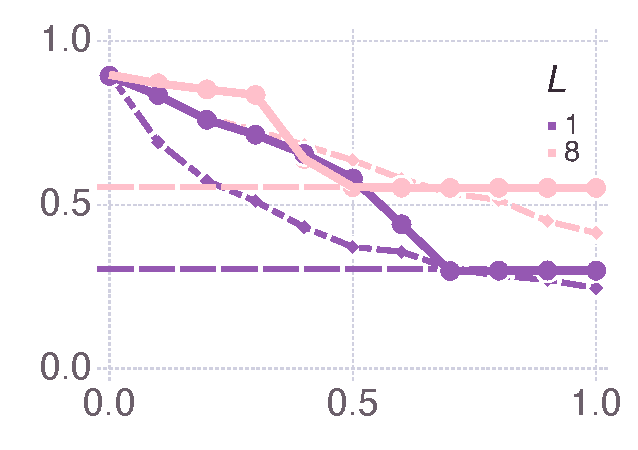
\includegraphics[width=\textwidth]{Figures/mean_prev_net_payoff_over_u_lowpayoff=0.1_nbehaviors=4.pdf}
    \end{minipage}\noindent
	\begin{minipage}{3.75in}%
      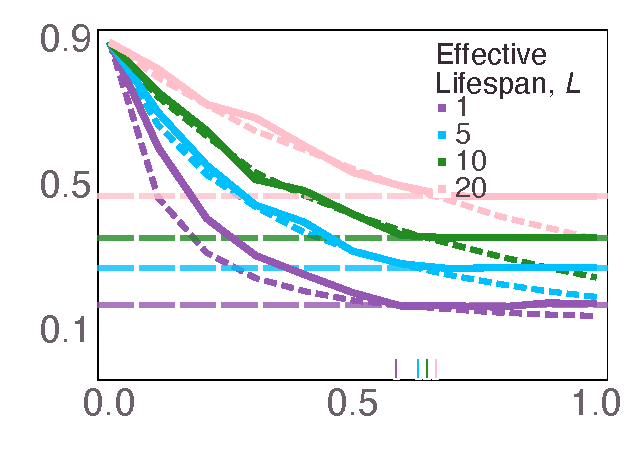
\includegraphics[width=\textwidth]{Figures/mean_prev_net_payoff_over_u_lowpayoff=0.1_nbehaviors=10.pdf}
    \end{minipage}~\\[0.5em]

    \begin{minipage}{3.75in}
    \begin{rotate}{90}
      {\parbox{2.5in}{
          \centering
          \vspace{-2.5em} {\huge$ \pilow = 0.45$} \\
          {\begin{rotate}{-90}{\huge $\frac{\meanpi}{L}$}\hspace{3em}\end{rotate}}
      }}
    \end{rotate}%
    \hspace{2em}
      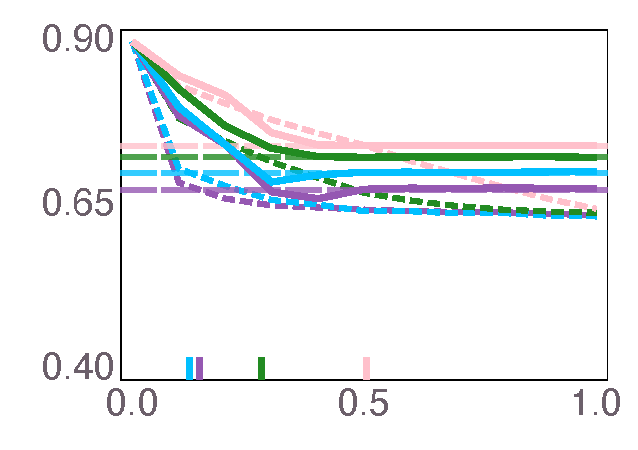
\includegraphics[width=\textwidth]{Figures/mean_prev_net_payoff_over_u_lowpayoff=0.45_nbehaviors=2.pdf}
	\end{minipage}\noindent\hspace{1.25em}
	\begin{minipage}{3.75in}%
      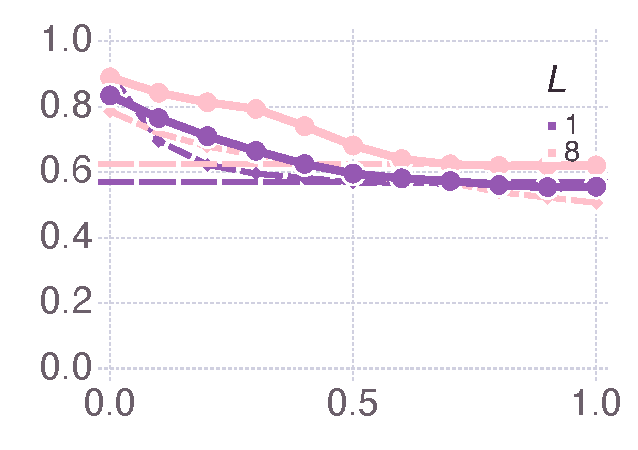
\includegraphics[width=\textwidth]{Figures/mean_prev_net_payoff_over_u_lowpayoff=0.45_nbehaviors=4.pdf}
    \end{minipage}\noindent
	\begin{minipage}{3.75in}%
      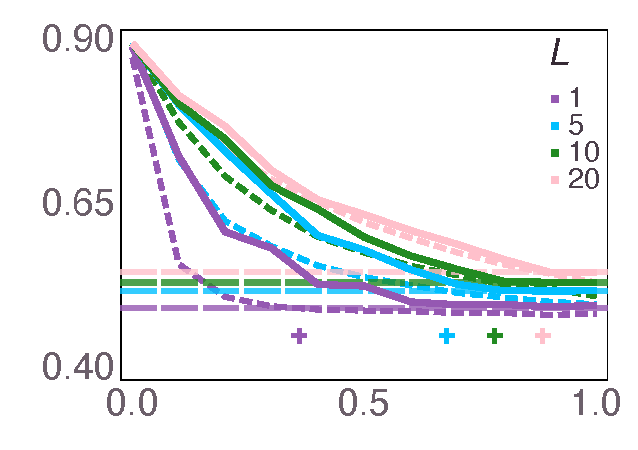
\includegraphics[width=\textwidth]{Figures/mean_prev_net_payoff_over_u_lowpayoff=0.45_nbehaviors=10.pdf}
    \end{minipage}~\\[0.5em]

    \begin{minipage}{3.75in}
    \begin{rotate}{90}
      {\parbox{2.5in}{
          \centering
          \vspace{-2.5em} {\huge$ \pilow = 0.8$} \\
          {\begin{rotate}{-90}{\huge $\frac{\meanpi}{L}$}\hspace{3em}\end{rotate}}
      }}
    \end{rotate}%
    \hspace{2em}
      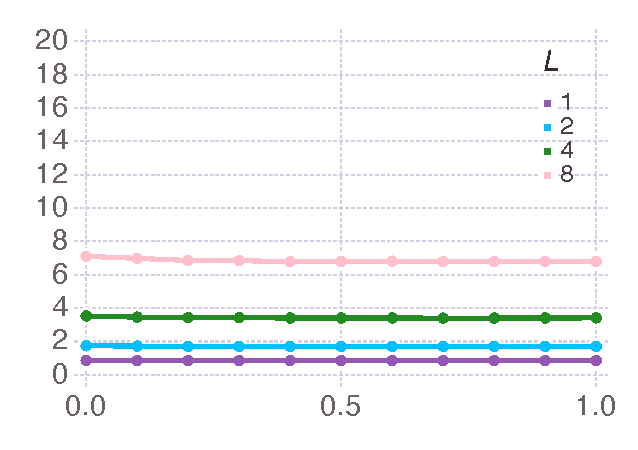
\includegraphics[width=\textwidth]{Figures/mean_prev_net_payoff_over_u_lowpayoff=0.8_nbehaviors=2.pdf}
        \\[-2.75em]
        \begin{center}
          {\hspace{3.25em} \huge $\quad u$}
      \end{center}
	  \end{minipage}\noindent\hspace{1.25em}
		\begin{minipage}{3.75in}%
		  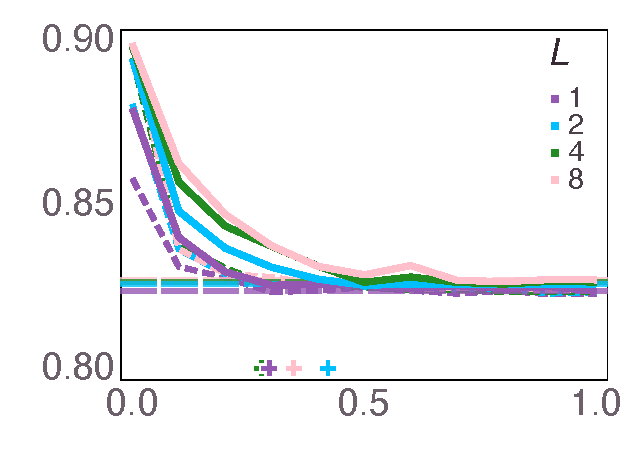
\includegraphics[width=\textwidth]{Figures/mean_prev_net_payoff_over_u_lowpayoff=0.8_nbehaviors=4.pdf}
		  \\[-2.75em]
	  \begin{center}
        {\huge $\quad u$}
      \end{center}
    \end{minipage}
	\begin{minipage}{3.75in}%
		  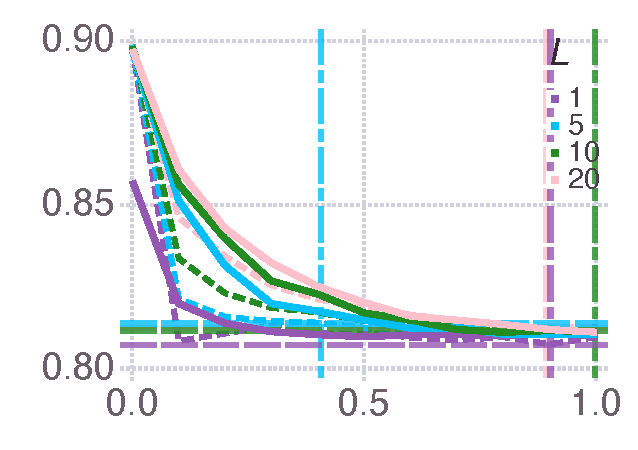
\includegraphics[width=\textwidth]{Figures/mean_prev_net_payoff_over_u_lowpayoff=0.8_nbehaviors=10.pdf}
		  \\[-2.75em]
	  \begin{center}
        {\huge $\quad u$}
      \end{center}
    \end{minipage} \\[2.5em]

    \begin{center}
       
\includegraphics[width=1.85in]{Figures/legendElements/dot.pdf}
       {\huge Average all-social population payoffs}  \\[1.125em]
       
\includegraphics[width=1.85in]{Figures/legendElements/ldash.pdf} 
       {\huge Average all-asocial population payoffs} \\[1.125em]
       
\includegraphics[width=1.85in]{Figures/legendElements/solid.pdf} 
       {\huge Simulated average population payoffs} \\[1.125em]
      {\Huge \textbf{+} \huge $u$ value where homogenous social and asocial payoffs
      are equal} 
    \end{center}

\end{document}


\documentclass[varwidth=true,crop=false]{standalone}
\usepackage[chatter]{rotating}
\usepackage{amssymb,amsmath}
\usepackage{pgfplots}

\usepackage{geometry}
\geometry{
paperwidth=8in,
paperheight=6.25in,
margin=0.25in
}

\newcommand{\pisub}[1]{\pi_{\mathrm{#1}}}
\newcommand{\pilow}{\pisub{low}}
\newcommand{\pihigh}{\pisub{high}}
\newcommand{\piI}{\langle \pisub{I} \rangle}
\newcommand{\piS}{\langle \pisub{S} \rangle}
\newcommand{\ledger}{\bar\pi_{ib}}

\newcommand{\meanvar}[1]{\langle #1 \rangle}
\newcommand{\meansl}{\meanvar{s}}
\newcommand{\meanpi}{\meanvar{\pi}}
\newcommand{\meansoc}{\meanvar{\pi_\mathrm{S}}}
\newcommand{\meanasoc}{\meanvar{\pi_\mathrm{A}}}
\newcommand{\meanT}{\meanvar{T}}

\newcommand{\bandit}{\text{Bandit}_b(0, 1)}

\begin{document}

    \begin{minipage}{3.75in}
      \centering
      {\hspace{5.25em}\huge $B = 4$}
    \end{minipage}%
    \begin{minipage}{3.75in}
      \centering
      {\hspace{2.0em}\huge $B = 10$}
    \end{minipage}~\\

    \begin{minipage}{3.75in}
    \begin{rotate}{90}
      {\parbox{2.5in}{
          \centering
          \vspace{-2.5em} {\huge$ \pilow = 0.1$} \\
          {\begin{rotate}{-90}{\huge $\frac{\meanT}{L}$}\hspace{3em}\end{rotate}}
      }}
    \end{rotate}%
    \hspace{2em}
      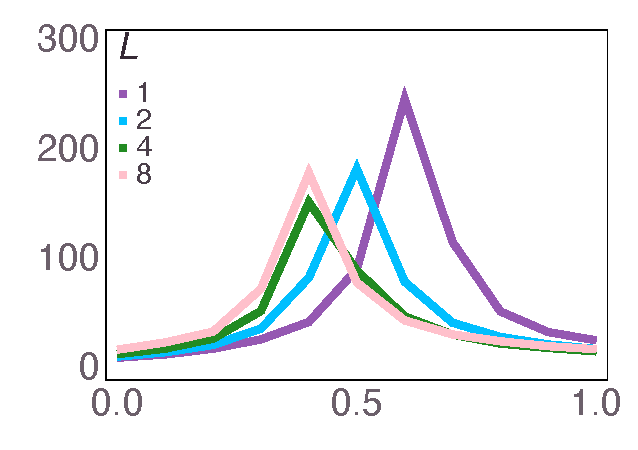
\includegraphics[width=\textwidth]{Figures/step_over_u_lowpayoff=0.1_nbehaviors=4.pdf}
    \end{minipage}\noindent\begin{minipage}{3.75in}%
      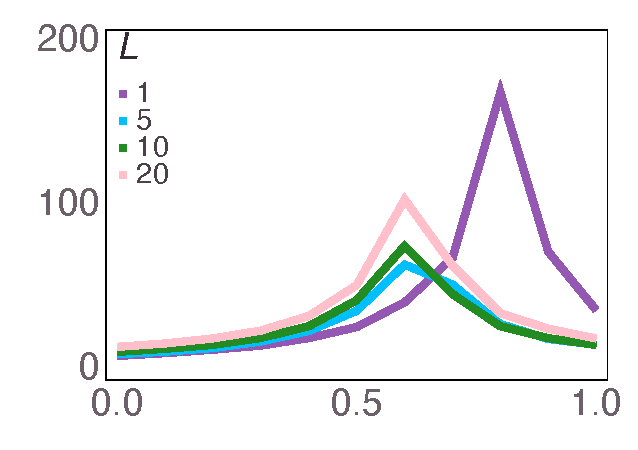
\includegraphics[width=\textwidth]{Figures/step_over_u_lowpayoff=0.1_nbehaviors=10.pdf}
    \end{minipage}~\\[0.5em]

    \begin{minipage}{3.75in}
    \begin{rotate}{90}
      {\parbox{2.5in}{
          \centering
          \vspace{-2.5em} {\huge$ \pilow = 0.45$} \\
          {\begin{rotate}{-90}{\huge $\frac{\meanT}{L}$}\hspace{3em}\end{rotate}}
      }}
    \end{rotate}%
    \hspace{2em}
      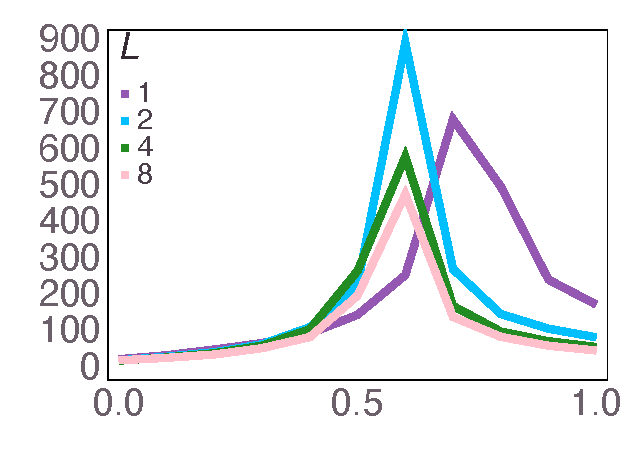
\includegraphics[width=\textwidth]{Figures/step_over_u_lowpayoff=0.45_nbehaviors=4.pdf}
        \\[-2.75em]
        \begin{center}
          {\hspace{3.25em} \huge $\quad u$}
      \end{center}
        \end{minipage}\noindent\begin{minipage}{3.75in}%
      \includegraphics[width=\textwidth]{Figures/step_over_u_lowpayoff=0.45_nbehaviors=10.pdf}
      \\[-2.75em]
      \begin{center}
        {\huge $\quad u$}
      \end{center}
    \end{minipage}
\end{document}

>>>>>>> 642146dabe76f30add3b2bafcd00edb4ef355867


\section{Discussion}

\begin{itemize}
  \item 
    Increasingly, engineers are blurring the line between humans and AI agents in designing
    effective interventions to the wicked problems we face
    today~\cite{Irrgang2021,Rolnick2022}.
  \item
    We have connected such augmented intelligence technologies as MARL to
    cultural evolution, which is a promising approach to addressing existential
    threats to life on Earth~\cite{Jones2021}.
\end{itemize}



% \section{Model}

% We developed an agent-based model of a society of $N$ individuals who each must decide
% which of $B$ behaviors to perform at each time step. Each behavior is a ``bandit'',
% a common modelling and experimental approach for representing behaviors with
% probabilistic payoffs~\cite{SuttonBartoBook, McElreath2005,Rendell2010,Schulz2019}. %Bandits are like  slot machines in a casino~\ref{fig:behaviorSelection}.
% Each behavior $b$ yields a payoff of 1 with probability $\pi_b$ and a payoff of zero
% otherwise; $\pi_b$ is therefore also the expected payoff of behavior $b$. Agents must
% decide which behavior to perform at each time step. To do this, agents 
% use an explore-exploit strategy to sometimes try the most profitable behavior
% they know about, and other times try alternatives that may pay off more reliably. 

% We operationalized uncertainty in four different ways: 
% (1) payoff ambiguity, $A_\pi$, which measures the difference
% between the optimal expected payoff behavior $\pisub{high}$ and the expected payoff
% of the other behaviors, $\pisub{low}$; 
% (2) environmental variability, $u$, the probability the optimal behavior changes from one generation to another; 
% (3) the number of possible behaviors, $B$; and 
% (4) the lifespan, or time steps per generation, $M$. 

% We ran the simulation for $T=1000$ time steps. At
% the end of each generation agents reproduce and then die off. 
% Those selected to reproduce
% pass on their boolean social learning trait, $s$, without mutation,
% which specifes whether agents learn socially. We developed a series of
% computational analyses where we systematically vary the uncertainty
% variables and observe the average prevalence of social learning trait $s$
% across agents and trials, which is our primary outcome measure, 
% denoted $\langle s \rangle$. 

% \subsection{Agents and their attributes}

% In each time step, $N$ agents---autonomous problem solvers---select 
% which behavior to perform based on their running tally of mean payoffs for 
% each available behavior. %information (Figure~\ref{fig:behaviorSelection}). 
% Agent $i$ tracks the mean payoff of each behavior $b$, denoted $\bar\pi_{ib}$, and
% a \emph{count} of how many times it has performed each behavior, denoted $c_{ib}$.
% $\bar\pi_{ib}$
% is initialized to 0 for all $b$ at model initialization for
% all agents, and after each generation for individual learner agents. Social
% learning agents' $\bar\pi_{ib}$ is initialized as that of its teacher selected
% through performance-biased oblique learning. Agent $i$'s accumulated payoffs
% from performing several behaviors over their lifetime of $M$ time steps is
% denoted $\pi_{i}$.


% \vspace{2em}

% \begin{table}[h]
%     \caption{Dynamic agent-level variables. Each has an implicit time dependence.}
%     \label{tab:modelParameters}
%     \centering \hspace{-3em}
%     \begin{tabular}{cp{4.0in}l} \toprule

%         Attribute & Description & Initial value \\ 

%         \midrule  

%         $s_i$  & Social learner trait: 1 if agent $i$ is social learner; 0 otherwise & 0
%         or 1 w/ equal prob. \\

%         $\bar\pi_{ib}$ & ``Ledger'': mean payoffs acquired via behavior $b$ by $i$ 
%                        & $B$-vector of floating-point zeros \\

%         $c_{ib}$ & Count of how many times agent $i$ performed $b$ 
%               & $B$-vector of integer zeros \\

%         $\pi_i$ & Net payoffs accumulated by $i$ within generation
%                                 & 0.0 \\
%         \bottomrule
%     \end{tabular}
% \end{table}

% \vspace{2em}




% \subsection{Modeling uncertainty}

% In our model uncertainty is a tunable consequence of four environmental features:
% \begin{enumerate}
%     \item 
%       We vary the frequency at which the optimal behavior changes, which we call
%       \emph{environmental variability}, $u$. At the start of each generation, with
%       probability $u$, a new behavior is assigned a payoff of $\pisub{high}$ while all
%       other behaviors are assigned a payoff of $\pisub{low}$. Otherwise, the same
%       behavior remains optimal across generations. 
%     \item We vary the latent expected payoffs yielded by the bandits. For simplicity,
%       we assume that in any given environmental state, there is one optimal behavior that
%       yields an expected payoff of $\pisub{high}$, while all other behaviors yield a 
%       payoff of $\pisub{low} < \pisub{high}$. As $\pilow$ increases towards 
%       $\pihigh$, uncertainty in the form of \emph{payoff ambiguity} also increases,
%       making it more difficult, and less rewarding, for agents to determine which
%       behavior is the optimal one.
%     \item We vary the total \emph{number of available behaviors}, $B$, which is a
%       source of uncertainty since agents are less likely to know which behavior yields high payoffs.  
%     \item Finally, we vary number of behavioral events per generation, $M$. This can be viewed as the \emph{effective lifespan} of an agent.  Decreasing this lifespan effectively increases the importance of each event for acquiring payoffs. When lifespans are short ($M$ is small), agents experience greater uncertainty about which behavior is optimal given the fewer learning opportunities.
% \end{enumerate}


% \subsection{Dynamics and evolution}

% Model dynamics can be split into three parts: initialization,
% \emph{intra}generational behavior and payoff accumulation, and
% \emph{inter}generational transmission of the social learning trait and oblique
% learning (Figure~\ref{fig:IntraInterGenerationalDynamics}). 
% The model runs that we analyze here were initialized with $N=100$ agents
% to randomly have the social learner trait or not, with no accumulated payoffs, and
% blank ``ledgers''. At each time step, agents select one of $B$ possible behaviors
% to perform, accumulating a payoff of 1 if the bandit pays off, and 0 if it does
% not---a bandit pays off with probability $\pihigh$ if it is the unique optimal
% behavior, or with probability $\pilow$ if it is one of $B-1$ non-optimal
% behaviors. Agents accumulate payoffs in this way for $M$ time steps in each
% generation. At the end of each generation, $N=100$ agents are randomly selected with
% replacement to reproduce (asexual, haploid reproduction), 
% weighted by their net payoffs over the generation,
% i.e., \emph{performance-biased} reproduction. Child agents then learn from 
% one teacher, selected again via a form of performance bias: a child agent chooses
% its teacher by first selecting a fully random subset of agents from the 
% parent generation as potential teachers, then selecting the one with the 
% greatest net payoffs among the subset. This process continues until $T=1000$
% time steps have elapsed \mt{this should probably be changed depending on $M$ so that
%     all analyses use the same number of generations. my informal checks have shown quick
% convergence, but i haven't tested b=4 and b=10 as much.}.

% \begin{figure}
%   \caption{Model dynamics are composed of two major parts: first, agents perform
%   behaviors for $M$ time steps in a single generation. Then agents reproduce
%   randomly, with more successful agents being more likely to reproduce. Newly
%   ``born'' social learner agents use success bias to select and learn from a chosen
%   teacher. Then, all agents from the previous generation die off, all new agents
%   begin a new generation, and the process continues until 1000 total time steps
%   have elapsed. Agents are initialized as ``blank slates''.}
%   \label{fig:IntraInterGenerationalDynamics}
%   \centering
%     \includegraphics[width=0.9\textwidth]{Figures/IntraInterGenerationalDynamics.pdf}
% \end{figure}


% \subsubsection{Initialization}

% Model initialization includes agent and environment initializations. Agents are
% randomly initialized to have the social learning trait or not, with equal 
% probability. Agent ``ledgers'' and behavior counts 
% are uniformly initialized to the no-knowledge,
% blank-slate case where all $\pi_{ib} = 0$ and $c_{ib} = 0$. Both the 
% ledger and behavior count vectors have $B$ entries, one for each
% behavior the environment affords. Net payoffs for
% the generation are also initialized to zero. All agents are initialized with
% the same softmax temperature, $\tau$, that guides their behavior selection 
% to be either more exploratory (greater $\tau$) or more exploitative of
% what agents believe to be the optimal behavior(s) (lesser $\tau$).

% The environment is initialized to have $B$ behaviors with one of them selected
% at random to be the optimal behavior, denoted $b^*$. Behavior $b^*$ is 
% initialized to have a probability $\pihigh$ of paying off 1. All other behaviors
% are initialized to have probability $\pilow$ of paying off 1. The modeler must
% specify the environmental variability, $u$, and the number of time steps per 
% generation, $M$. 


% \vspace{2em}
% \begin{table}[h]
%     \caption{Global environmental and cognitive initialization parameters.}
%     \label{tab:modelParameters}
%     \centering \hspace{-3em}
%     \begin{tabular}{cp{4.0in}l} \toprule

%         Symbol & Description & Values tested (bold$=$default) \\ 

%         \midrule  

%         $B$       & Number of possible behaviors (represented by ``bandits'') 
%                   & 2, 4, 10 \\

%         $\pihigh$ & Probability that the unique optimal behavior pays off 1 
%                 & \textbf{0.9} \\

%         $\pilow$ & Probability one of $B - 1$ non-optimal behaviors pays off 1 
%                  & 0.1, 0.45, 0.8 \\ 

%         $\tau$ & Softmax temp.; $\uparrow=$more exploration, $\downarrow=$more
%                     exploitation 
%                & 0.01, \textbf{0.1}, 1.0 \\
        
%         $u$    & Probability optimal behavior changes between generations 
%                & 0.0, 0.1, \ldots, 1.0 \\

%         $M$    & Number of time steps per generation & 1, $B/2$, $B$, $2B$ \\

%         $N_T$    & Number of teachers to pool, from which best selected 
%                  & \textbf{5} \mt{TODO: Test more for sensitivity analysis?} \\

            
               
%         \bottomrule
%         \end{tabular} 
% \end{table}
% \vspace{2em}


% \subsubsection{Intra-generational behaviors and payoffs}

% Each generation begins with agents initialized either by the $t=0$ initialization
% outlined above, or initialized via inter-generational reproduction and learning,
% described in detail below. Within generations, there is no social learning.
% At each time step within a generation, agents select a behavior to perform
% using the softmax algorithm, then update their ledgers $\bar\pi_{ib}$ and behavior
% counts $c_{ib}$. If 
% the chosen bandit pays off for an agent, its net payoff is incremented by one,
% $\pi'_i \leftarrow \pi_i + 1$. This process continues for $M$ time steps, 
% when reproduction, learning, and die-off occur, re-initializing the next 
% generation for performing $M$ behaviors selected via this same process.

% At each time step, 
% agent $i$ chooses behavior $b$ at random, with each behavior
% weighted by the softmax function applied to that behavior's observed mean payoff
% relative to all mean payoffs in the ledger,
% \begin{equation}
%   \Pr(i \text{ chooses behavior } b) = \frac{\exp(\bar\pi_{ib}
%   / \tau) }{ \sum_{b=1}^B \exp(\bar\pi_{ib} / \tau)}.
% \end{equation}  
% Softmax behavior selection is a
% biologically plausible model of behavior~\cite{Schulz2019} 
% that enables agents to explore
% alternative behaviors sometimes and exploit the best observed behavior other times,
% in accordance with Luce's choice axiom~\cite{Luce1959},.
% The parameter $\tau$ specifies how frequently alternative behaviors are
% explored versus how frequently the best observed behaviors are 
% exploited. Greater $\tau$ means more frequent exploration, lesser $\tau$ means
% more frequent exploitation. We set $\tau = 0.1$ for
% all computational analyses presented in the main paper. We (WILL HAVE) performed
% sensitivity analyses and found a weak dependence on $\tau$ that does not affect our
% main conclusions.

% When agent $i$ performs behavior $b$, $i$'s behavior count 
% is incremented by 1, $c'_{ib} \leftarrow c_{ib} + 1$. Agent $i$'s ledger of mean 
% payoffs are updated % from $\bar\pi_{ib}$ to $\bar\pi_{ib}'$
% using exponential weighted averaging, 

% \begin{equation}
%   \bar\pi_{ib}' = \bar\pi_{ib} +
%     \frac{\mathrm{Bandit_{b}(0, 1)} - \bar\pi_{ib}}{c_{ib}'},
% \end{equation}
% where 
% $\mathrm{Bandit}_{b}(0, 1)$
% is 0 or 1 depending on the result of the bandit draw for behavior $b$. 


% \subsubsection{Inter-generational inheritance and social learning}

% Every $M$ time steps, agents from the current generation reproduce, teach,
% and die, while the next generation to perform the next $M$ time steps learns
% from one teacher from the previous generation if they inherited the social 
% learner trait. Inter-generational dynamics thus depend on 
% two payoff-biased selection mechanisms: reproducer selection
% and teacher selection. 

% $N$ reproducers are sampled from the population with
% replacement weighted by net payoffs, i.e., at each of $N$ draws for a parent,
% \begin{equation}
%   \Pr(\text{Agent $i$ chosen for reproduction}) = \frac{\pi_i}{\sum_{i=1}^N \pi_i}.
% \end{equation}
% \noindent
% We sample with replacement to allow for more successful agents to have multiple
% offspring. Child agents inherit their parents' social learning trait, so 
% all social learner parents spawn social learner offspring, and parents lacking
% the trait spawn offspring lacking the trait. 

% Child agents with the social learning trait then must select and learn from a
% teacher from their parent's generation, including possibly their parent.
% Child agents give no preference to whether potential teachers are social 
% learners. A child selects a teacher by first selecting a pool of $N_T = 5$ potential
% teachers. Among this pool, each child selects the teacher with the greatest
% net payoffs. In case of a tie the teacher is chosen at random from those with
% the shared maximum net payoff. 

% Social learner child agents each acquire their teacher's ledger, and all social
% learner children behavior counts are reset to 1 to limit ledger values to be between
% 0 and 1. Child agents without the social learner trait have all ledger and behavior
% count values re-initialized to 0. At this point the re-initialized child agents
% engage in behavior selection and payoff accumulation described above. 


% \subsection{Computational analyses}

% We manipulated environmental uncertainty parameters described above, $u$,
% $\pisub{low}$, $B$, and $M$, to examine their effects on our
% main outcome measure, the prevalence of social learning $s$. For each parameter setting
% in our analysis we calculated the average value of $s$ at the final time step
% of $T=1000$ across 100 runs for each combination of uncertainty parameter values.

% To analyze the effect of various forms of uncertainty on social learning 
% prevalence in our Analysis, we initialized several model runs with
% different uncertainty parameters $u$, $\pisub{\mathrm{low}}$, $B$,
% and $M$. We varied $u \in \{0.0, 0.1, \ldots, 1.0\}$ for each combination of
% the following parameters:
% $\pisub{low} \in \{0.1, 0.5, 0.8\}$, $B \in \{2, 4, 10\}$, $M \in \{B/2, B, 2B\}$.

% \subsubsection{Outcome variables}

% Our primary outcome variable is the mean prevalence of the social learning
% trait over $N=100$ agents over 1000 trials at the final time step of each trial,
% denoted $\meansl$.
% Typically at the final time step all agents either have the social learning
% trait or do not (see Supplement for a presentation of time series collections
% and histograms of outcomes for
% a representative sampling of variables \mt{TODO}).

% \begin{table}[h]
%     \caption{Global environmental and cognitive initialization parameters.}
%     \label{tab:modelParameters}
%     \centering \hspace{-3em}
%     \begin{tabular}{cp{4.0in}l} \toprule

%         Symbol & Description & Values \\ 

%         \midrule  

%         $\meansl$ & Mean social learning prevalence over agents and trials
%                   & $\in [0.0, 1.0]$ \\

%         $p_{\text{opt}}$ & Fraction of population performing optimal behavior
%                          & $\in [0.0, 1.0]$ \\

%         \texttt{count}$(b_i)$ & Number of agents performing behavior $b$ 
%                               & Behavior-count key-value pairs\\
%         \bottomrule
%     \end{tabular}
% \end{table}


% \section{Analysis}

% We analyzed the outcomes of model runs across systematically varied uncertainty
% parameters over 1000 trials for each parameter setting. 
% We observed complex outcomes where the effects of uncertainty parameters
% were highly dependent on one another as measured by the mean prevalence of
% social learning, $\meansl$, across trials for each parameter setting. 
% The prevalence of social learning
% generally decreased with environmental variability, $u$, as expected from standard
% models of social learning evolution. However, the shape of the decrease was not
% uniform (Figure~\ref{fig:evolutionOfSL}). 
% We observed that social learning did in fact enable populations to 
% do better than individual learners, but only when (multi-dimensional) uncertainty 
% were sufficiently limited (Figure~\ref{fig:meanNetPayoffs}).


% \subsection{Evolution of social learning under uncertainty}
% The shape of the decrease from all agents
% always becoming social learners ($\meansl = 1.0$) to 
% all agents always becoming individual learners ($\meansl = 0.0$)
% is heterogeneous. We identified patterns in this heterogeneity that inform our
% understanding of when and how social learning is advantageous, and when 
% and why individual learning is advantageous. 
% Changes in the uncertainty parameters ($\pilow$, $B$, $L$) 
% result in the following changes in the shape of the transition from $\meansl = 1.0$ 
% to $\meansl = 0.0$: (1) the transition
% occurs at different critical values of $u$; and (2) the transition occurs
% with greater or lesser rapidity over $u$. 
% For instance, when $B=2$, $\pilow = 0.1$, and $L=8$, $\meansl$ goes from 1 to 
% 0 starting at $u=0.1$ and reaches 0 at $u=0.3$ (Figure~\ref{fig:evolutionOfSL},
% top left). When we increased $B=4$ (Figure~\ref{fig:evolutionOfSL}, top center), the
% transition from $\meansl = 1$ to 0 begins at $u=0.3$. When $B=4$, $\pilow=0.1$,
% and $L=1$ the transition from $\meansl=1$ to 0 begins at $u=0.3$ but does not
% reach 0 until $u \approx 0.9$ (again Figure~\ref{fig:evolutionOfSL}, top center).

% We can draw some conclusions about the evolution of social learning by analyzing the
% location and shape of the suppression of social learning as $u$ was increased.
% First, let us observe some general trends. Increased $\pilow$ generally
% flattened the suppression of social learning as $u$ increased.  
% Increased $B$ tended to increase the critical value of $u$ at which the 
% system transitions from favoring social learning to favor individual learning.  
% Increased $L$ generally sharpened the suppression of social learning.
% Within each of these broad trends over the uncertainty parameters are several
% details that depend on context as defined by the values of the other uncertainty
% parameters.

% When $\pilow$ was increased, the suppression of social learning was, in
% general, less rapid as $u$ increased. This effect is particularly acute when
% $\pilow = 0.8$, which is very nearly equal to the expected value of the optimal
% payoff, $\pihigh = 0.9$. When $\pilow = 0.8$ $\meansl$ never actually reaches 
% 1 or 0 for any parameter settings. The suppression of social learning in this
% case is approximately linear, if there is selection at all. When $\pilow = 0.8$
% and $L = 1$ there is little to no selection across $B$, 
% so populations evolve randomly towards $\meansl = 1$ or $\meansl = 0$. 

% Increased $B$ generally led to increased critical $u$ at which social learning
% starts to be suppresed. When payoffs are not ambiguous ($\pilow = 0.1$), the the
% suppression of social learning starts at $u \approx 0.1$ for $B=2$; at $u \approx
% 0.3$ when $B=4$; and at $u \approx 0.5$ when $B=10$.  When payoffs are more
% ambiguous ($\pilow = 0.45,0.8$), increased $B$ also led to a flattening of the
% suppression of social learning when $L=1$. 

% The general effect of $L$ is to increase the rapidity of the suppression of social
% learning via the strengthening of selection pressure since longer-lived agents
% build up stronger priors over their lifetimes. If it is advantageous to
% learn socially, this will be reliably detected. Inversely, decreased $L$
% can weaken selection pressure since agents cannot amass useful information when
% $L$ is small. This is most extreme when $\pilow = 0.8$ and there is little to
% no selection for or against social learning when $L=1$. However, decreased $L$ can
% also delay the suppression of social learning as $u$ increases, since social
% learning provdes agents with the possibility of learning what the optimal behavior
% might be.  Even when $u$ was large, agents with a lifespan of 1 more often evolved
% to be social learners because social learning was to be preferred over random
% chance.


% \subsection{Social learning capacity increases payoffs}

% For social learning to evolve, it must improve upon individual learning. 
% We found that different parameter settings indeed change how advantageous social learning
% is compared to individual learning (Figure~\ref{fig:meanNetPayoffs}). 
% To analyze the effect of uncertainty on
% payoffs, it is useful to identify some constant reference values which we will
% use to evaluate the benefit of social learning. First, the optimal expected payoff
% is the optimal behavior payoff times the lifespan, which we can denote
% $\langle \pi^*(L) \rangle = L\cdot\pihigh$. The expected base payoff by chance is 
% $\langle \pi_{\text{base}} \rangle = L \left[ (B - 1) \pilow + \pihigh \right]$, which
% an agent would receive on average from performing purely random behaviors. 
% Most importantly for understanding the benefit and evolution of social learning,
% we calculated by simulation the expected payoff to individual learners for
% each triplet ($\pilow$, $B$, $L$), which we denote $\langle \pi_I \rangle$
% and plot for reference in Figure~\ref{fig:meanNetPayoffs}. Note $\langle \pi_I
% \rangle$ is insensitive to $u$, which only affects the benefit of social
% learning.

% We observe across parameter settings that social learning outperforms
% individual learning when $u$ is small. In fact, when $u=0.0$, social learning 
% enables each new generation to know the optimal behavior and achieve the maximum
% expected payoff for their lifespan, $\langle \pi^*(L) \rangle$. 
% However, in some cases, even when $u$ is small, 
% the returns on social learning are truly marginal due to 
% relatively high, uniform expected payoffs whether or not agents identify the optimal
% behavior, especially when $\pilow = 0.8$. In intermediate cases, examining the decay
% of the benefit of social learning informs our understanding of social learning
% evolution analyzed above.  As our analysis of social learning evolution suggested,
% social learning is only beneficial up to a point. When $\pilow=0.1$, increasing $B$
% led both to larger differences between 

% \subsection{Evolutionary outcomes vary in their certainty} 

% Finally, we found that the \emph{evolutionary uncertainty} of the system increases
% around the values of $u$ where $\meansl$ goes from 1 to 0. 
% In one sense
% To confirm and expand our analysis of this uncertainty, we 
% also measured environmental uncertainty in terms of the
% expected number of time steps to convergence, $\langle T \rangle$. Evolutionary
% uncertainty is an outcome measure---an emergent form of uncertainty due to
% weak selection pressures. When 
% $\meansl \approx 0.5$ this means that approximately equal numbers of trials
% ended with all agents as social learners as they ended with all agents 
% individual learners. We found that increased $\pilow$
% tended to increase the overall uncertainty in terms of $\langle T \rangle$.
% Increasing $B$ also increased the $u$ at which $\langle T \rangle$ peaked.
% This indicates the evolutionary system is significantly less certain of 
% which behavior is optimal around critical uncertainty parameter ensembles.

% \mt{interpret this further}



% \documentclass[varwidth=true,crop=false]{standalone}
\usepackage[chatter]{rotating}
\usepackage{amssymb,amsmath}
\usepackage{pgfplots}

\usepackage{geometry}
\geometry{
paperwidth=12in,
paperheight=12in,
margin=0.25in
}

\newcommand{\pisub}[1]{\pi_{\mathrm{#1}}}
\newcommand{\pilow}{\pisub{low}}
\newcommand{\pihigh}{\pisub{high}}
\newcommand{\piI}{\langle \pisub{I} \rangle}
\newcommand{\piS}{\langle \pisub{S} \rangle}
\newcommand{\ledger}{\bar\pi_{ib}}

\newcommand{\meanvar}[1]{\langle #1 \rangle}
\newcommand{\meansl}{\meanvar{s}}
\newcommand{\meanpi}{\meanvar{\pi}}
\newcommand{\meansoc}{\meanvar{\pi_\mathrm{S}}}
\newcommand{\meanasoc}{\meanvar{\pi_\mathrm{A}}}
\newcommand{\meanT}{\meanvar{T}}

\newcommand{\bandit}{\text{Bandit}_b(0, 1)}

\begin{document}
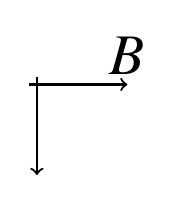
\begin{tikzpicture}
      \draw[->,thick] (-.1,0)--(1.15,0) node[above]
        {\huge $B$};
        % {Number of behaviors $B$};
      \draw[->,thick] (0,.1)--(0,-1.15) node[below]
        {\huge $\pilow$};
        % {Low payoff frequency $\pilow$};
	  \end{tikzpicture}~\\[-2em]

    \begin{minipage}{3.75in}
      \centering
      {\hspace{5.25em}\huge $B = 2$}
    \end{minipage}%
    \begin{minipage}{3.75in}
      \centering
      {\hspace{1.0em}\huge $B = 4$}
    \end{minipage}%
    \begin{minipage}{3.75in}
      \centering
      {\hspace{2.0em}\huge $B = 10$}
    \end{minipage}~\\

    \begin{minipage}{3.75in}
    \begin{rotate}{90}
      {\parbox{2.5in}{
          \centering
          \vspace{-2.5em} {\huge$ \pilow = 0.1$} \\
          {\begin{rotate}{-90}{\huge $\meansl$}\hspace{3em}\end{rotate}}
      }}
    \end{rotate}%
    \hspace{2em}
      \includegraphics[width=\textwidth]{mean_social_learner_over_u_lowpayoff=0.1_nbehaviors=2.pdf}
    \end{minipage}\noindent\hspace{1.25em}
	\begin{minipage}{3.75in}%
      \includegraphics[width=\textwidth]{mean_social_learner_over_u_lowpayoff=0.1_nbehaviors=4.pdf}
    \end{minipage}\noindent
	\begin{minipage}{3.75in}%
      \includegraphics[width=\textwidth]{mean_social_learner_over_u_lowpayoff=0.1_nbehaviors=10.pdf}
    \end{minipage}~\\[0.5em]

    \begin{minipage}{3.75in}
    \begin{rotate}{90}
      {\parbox{2.5in}{
          \centering
          \vspace{-2.5em} {\huge$ \pilow = 0.45$} \\
          {\begin{rotate}{-90}{\huge $\meansl$}\hspace{3em}\end{rotate}}
      }}
    \end{rotate}%
    \hspace{2em}
      \includegraphics[width=\textwidth]{mean_social_learner_over_u_lowpayoff=0.45_nbehaviors=2.pdf}
	\end{minipage}\noindent\hspace{1.25em}
	\begin{minipage}{3.75in}%
      \includegraphics[width=\textwidth]{mean_social_learner_over_u_lowpayoff=0.45_nbehaviors=4.pdf}
    \end{minipage}\noindent
	\begin{minipage}{3.75in}%
      \includegraphics[width=\textwidth]{mean_social_learner_over_u_lowpayoff=0.45_nbehaviors=10.pdf}
    \end{minipage}~\\[0.5em]

    \begin{minipage}{3.75in}
    \begin{rotate}{90}
      {\parbox{2.5in}{
          \centering
          \vspace{-2.5em} {\huge$ \pilow = 0.8$} \\
          {\begin{rotate}{-90}{\huge $\meansl$}\hspace{3em}\end{rotate}}
      }}
    \end{rotate}%
    \hspace{2em}
      \includegraphics[width=\textwidth]{mean_social_learner_over_u_lowpayoff=0.8_nbehaviors=2.pdf}
        \\[-2.75em]
        \begin{center}
          {\hspace{3.25em} \huge $\quad u$}
      \end{center}
	  \end{minipage}\noindent\hspace{1.25em}
		\begin{minipage}{3.75in}%
		  \includegraphics[width=\textwidth]{mean_social_learner_over_u_lowpayoff=0.8_nbehaviors=4.pdf}
		  \\[-2.75em]
	  \begin{center}
        {\huge $\quad u$}
      \end{center}
    \end{minipage}
	\begin{minipage}{3.75in}%
		  \includegraphics[width=\textwidth]{mean_social_learner_over_u_lowpayoff=0.8_nbehaviors=10.pdf}
		  \\[-2.75em]
	  \begin{center}
        {\huge $\quad u$}
      \end{center}
	\end{minipage}%
\end{document}


% \documentclass[varwidth=true,crop=false]{standalone}
\usepackage[chatter]{rotating}
\usepackage{amssymb,amsmath}
\usepackage{pgfplots}

\usepackage{geometry}
\geometry{
paperwidth=12in,
paperheight=12in,
margin=0.25in
}

\newcommand{\pisub}[1]{\pi_{\mathrm{#1}}}
\newcommand{\pilow}{\pisub{low}}
\newcommand{\pihigh}{\pisub{high}}
\newcommand{\piI}{\langle \pisub{I} \rangle}
\newcommand{\piS}{\langle \pisub{S} \rangle}
\newcommand{\ledger}{\bar\pi_{ib}}

\newcommand{\meanvar}[1]{\langle #1 \rangle}
\newcommand{\meansl}{\meanvar{s}}
\newcommand{\meanpi}{\meanvar{\pi}}
\newcommand{\meansoc}{\meanvar{\pi_\mathrm{S}}}
\newcommand{\meanasoc}{\meanvar{\pi_\mathrm{A}}}
\newcommand{\meanT}{\meanvar{T}}

\newcommand{\bandit}{\text{Bandit}_b(0, 1)}

\begin{document}
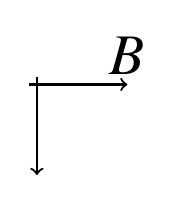
\begin{tikzpicture}
      \draw[->,thick] (-.1,0)--(1.15,0) node[above]
        {\huge $B$};
        % {Number of behaviors $B$};
      \draw[->,thick] (0,.1)--(0,-1.15) node[below]
        {\huge $\pilow$};
        % {Low payoff frequency $\pilow$};
	  \end{tikzpicture}~\\[-2em]

    \begin{minipage}{3.75in}
      \centering
      {\hspace{5.25em}\huge $B = 2$}
    \end{minipage}%
    \begin{minipage}{3.75in}
      \centering
      {\hspace{1.0em}\huge $B = 4$}
    \end{minipage}%
    \begin{minipage}{3.75in}
      \centering
      {\hspace{2.0em}\huge $B = 10$}
    \end{minipage}~\\

    \begin{minipage}{3.75in}
    \begin{rotate}{90}
      {\parbox{2.5in}{
          \centering
          \vspace{-2.5em} {\huge$ \pilow = 0.1$} \\
          {\begin{rotate}{-90}{\huge $\frac{\meanpi}{L}$}\hspace{3em}\end{rotate}}
      }}
    \end{rotate}%
    \hspace{2em}
      \includegraphics[width=\textwidth]{Figures/mean_prev_net_payoff_over_u_lowpayoff=0.1_nbehaviors=2.pdf}
    \end{minipage}\noindent\hspace{1.25em}
	\begin{minipage}{3.75in}%
      \includegraphics[width=\textwidth]{Figures/mean_prev_net_payoff_over_u_lowpayoff=0.1_nbehaviors=4.pdf}
    \end{minipage}\noindent
	\begin{minipage}{3.75in}%
      \includegraphics[width=\textwidth]{Figures/mean_prev_net_payoff_over_u_lowpayoff=0.1_nbehaviors=10.pdf}
    \end{minipage}~\\[0.5em]

    \begin{minipage}{3.75in}
    \begin{rotate}{90}
      {\parbox{2.5in}{
          \centering
          \vspace{-2.5em} {\huge$ \pilow = 0.45$} \\
          {\begin{rotate}{-90}{\huge $\frac{\meanpi}{L}$}\hspace{3em}\end{rotate}}
      }}
    \end{rotate}%
    \hspace{2em}
      \includegraphics[width=\textwidth]{Figures/mean_prev_net_payoff_over_u_lowpayoff=0.45_nbehaviors=2.pdf}
	\end{minipage}\noindent\hspace{1.25em}
	\begin{minipage}{3.75in}%
      \includegraphics[width=\textwidth]{Figures/mean_prev_net_payoff_over_u_lowpayoff=0.45_nbehaviors=4.pdf}
    \end{minipage}\noindent
	\begin{minipage}{3.75in}%
      \includegraphics[width=\textwidth]{Figures/mean_prev_net_payoff_over_u_lowpayoff=0.45_nbehaviors=10.pdf}
    \end{minipage}~\\[0.5em]

    \begin{minipage}{3.75in}
    \begin{rotate}{90}
      {\parbox{2.5in}{
          \centering
          \vspace{-2.5em} {\huge$ \pilow = 0.8$} \\
          {\begin{rotate}{-90}{\huge $\frac{\meanpi}{L}$}\hspace{3em}\end{rotate}}
      }}
    \end{rotate}%
    \hspace{2em}
      \includegraphics[width=\textwidth]{Figures/mean_prev_net_payoff_over_u_lowpayoff=0.8_nbehaviors=2.pdf}
        \\[-2.75em]
        \begin{center}
          {\hspace{3.25em} \huge $\quad u$}
      \end{center}
	  \end{minipage}\noindent\hspace{1.25em}
		\begin{minipage}{3.75in}%
		  \includegraphics[width=\textwidth]{Figures/mean_prev_net_payoff_over_u_lowpayoff=0.8_nbehaviors=4.pdf}
		  \\[-2.75em]
	  \begin{center}
        {\huge $\quad u$}
      \end{center}
    \end{minipage}
	\begin{minipage}{3.75in}%
		  \includegraphics[width=\textwidth]{Figures/mean_prev_net_payoff_over_u_lowpayoff=0.8_nbehaviors=10.pdf}
		  \\[-2.75em]
	  \begin{center}
        {\huge $\quad u$}
      \end{center}
    \end{minipage} \\[2.5em]

    \begin{center}
       \includegraphics[width=1.85in]{Figures/legendElements/dot.pdf}
       {\huge Average all-social population payoffs}  \\[1.125em]
       \includegraphics[width=1.85in]{Figures/legendElements/ldash.pdf} 
       {\huge Average all-asocial population payoffs} \\[1.125em]
       \includegraphics[width=1.85in]{Figures/legendElements/solid.pdf} 
       {\huge Simulated average population payoffs} \\[1.125em]
      {\Huge \textbf{+} \huge $u$ value where homogenous social and asocial payoffs
      are equal} 
    \end{center}

\end{document}


% \documentclass[varwidth=true,crop=false]{standalone}
\usepackage[chatter]{rotating}
\usepackage{amssymb,amsmath}
\usepackage{pgfplots}

\usepackage{geometry}
\geometry{
paperwidth=8in,
paperheight=6.25in,
margin=0.25in
}

\newcommand{\pisub}[1]{\pi_{\mathrm{#1}}}
\newcommand{\pilow}{\pisub{low}}
\newcommand{\pihigh}{\pisub{high}}
\newcommand{\piI}{\langle \pisub{I} \rangle}
\newcommand{\piS}{\langle \pisub{S} \rangle}
\newcommand{\ledger}{\bar\pi_{ib}}

\newcommand{\meanvar}[1]{\langle #1 \rangle}
\newcommand{\meansl}{\meanvar{s}}
\newcommand{\meanpi}{\meanvar{\pi}}
\newcommand{\meansoc}{\meanvar{\pi_\mathrm{S}}}
\newcommand{\meanasoc}{\meanvar{\pi_\mathrm{A}}}
\newcommand{\meanT}{\meanvar{T}}

\newcommand{\bandit}{\text{Bandit}_b(0, 1)}

\begin{document}

    \begin{minipage}{3.75in}
      \centering
      {\hspace{5.25em}\huge $B = 4$}
    \end{minipage}%
    \begin{minipage}{3.75in}
      \centering
      {\hspace{2.0em}\huge $B = 10$}
    \end{minipage}~\\

    \begin{minipage}{3.75in}
    \begin{rotate}{90}
      {\parbox{2.5in}{
          \centering
          \vspace{-2.5em} {\huge$ \pilow = 0.1$} \\
          {\begin{rotate}{-90}{\huge $\frac{\meanT}{L}$}\hspace{3em}\end{rotate}}
      }}
    \end{rotate}%
    \hspace{2em}
      \includegraphics[width=\textwidth]{Figures/step_over_u_lowpayoff=0.1_nbehaviors=4.pdf}
    \end{minipage}\noindent\begin{minipage}{3.75in}%
      \includegraphics[width=\textwidth]{Figures/step_over_u_lowpayoff=0.1_nbehaviors=10.pdf}
    \end{minipage}~\\[0.5em]

    \begin{minipage}{3.75in}
    \begin{rotate}{90}
      {\parbox{2.5in}{
          \centering
          \vspace{-2.5em} {\huge$ \pilow = 0.45$} \\
          {\begin{rotate}{-90}{\huge $\frac{\meanT}{L}$}\hspace{3em}\end{rotate}}
      }}
    \end{rotate}%
    \hspace{2em}
      \includegraphics[width=\textwidth]{Figures/step_over_u_lowpayoff=0.45_nbehaviors=4.pdf}
        \\[-2.75em]
        \begin{center}
          {\hspace{3.25em} \huge $\quad u$}
      \end{center}
        \end{minipage}\noindent\begin{minipage}{3.75in}%
      \includegraphics[width=\textwidth]{Figures/step_over_u_lowpayoff=0.45_nbehaviors=10.pdf}
      \\[-2.75em]
      \begin{center}
        {\huge $\quad u$}
      \end{center}
    \end{minipage}
\end{document}



% \section{Discussion}


\bibliographystyle{apacite}

\setlength{\bibleftmargin}{.125in}
\setlength{\bibindent}{-\bibleftmargin}

% \bibliography{/Users/mt/workspace/Writing/library.bib}
\bibliography{this.bib}


\appendix

\section{Appendix}



\subsection{Convergence information}

\begin{table}[h]
  \caption{Max. iterations = 5000.}
  \label{tab:convergence}
  \centering
  \begin{tabular}{cccc} \toprule
    $B$ & \# not at fixation & \# total series & Pct. not fixated \\
    \midrule  
    2  & 0  & 132000 & 0.0 \% \\
    4  & 0  & 132000 & 0.0 \% \\
    10 & 44 & 132000 & 0.00033  \% \\
    \bottomrule
  \end{tabular} 
\end{table}


\end{document}
